\documentclass[11pt]{gsasthesis} % 10,11 and 12pt fonts allowed

%%%%%%%%%%%%%%%% PACKAGES YOU PROBABLY WANT %%%%%%%%%%%%%%%%
% Include packages you want. The gsasthesis style file already includes
% packages "setspace" and "tocbibind".

\usepackage{etex} % extend the number of registers

% GSAS: "all margins should be at least 1 inch."
\usepackage[margin={1.2in}]{geometry}
% If you want asymmetric margins for two-sided documents, use the "twoside"
% option, as in
% \usepackage[top=1in,bottom=1.5in,left=1in,right=1.5in,twoside]{geometry} The
% left and right options become inner and outer margins The default horizontal
% latex margin ratio is 2:3. The default vertical top:bottom margin ratio is 2:3
% also. You can also set it directly by passing the hmarginratio option to the
% geometry package, as in
% \usepackage[top=1in,left=1in,vmarginratio=2:3,hmarginratio=2:5,twoside]{geometry}

% Appendix package. Not necessary, but it does make managing appendices easier
\usepackage[titletoc]{appendix}

%%%%%%%%%%%%%%%% PACKAGES MAY WANT %%%%%%%%%%%%%%%%

% sideways tables and figures
\usepackage{rotating}

% tables that spill over multiple pages
\usepackage{longtable}

% references
\usepackage{natbib}

% fonts that are nicer than defaults
\usepackage[sc]{mathpazo}
\usepackage{courier}

% Use 8-bit encoding that has 256 glyphs, pretty please
\usepackage[utf8]{inputenc}
\usepackage[T1]{fontenc}

% babel is required for blindtext, which generates random text
\usepackage[english]{babel}
\usepackage{blindtext}

% math support
\usepackage{amsmath}

% Slightly tweak font spacing for aesthetics
\usepackage{microtype}

% You need the footmisc package with the stable option if you want to have
% footnotes inside section titles, for example to say that a particular chapter
% has been co-authored with someone. The multiple option ensures that there is a
% comma between two consecutive footnotes
\usepackage[stable,multiple]{footmisc}


% Nicer captions
\RequirePackage[font=small,format=plain,labelfont=bf,textfont=it]{caption}
\addtolength{\abovecaptionskip}{1ex}
\addtolength{\belowcaptionskip}{1ex}


%%%%%%%%%%%%%%%% COMPULSORY FIELDS %%%%%%%%%%%%%%%%

\title{Rising from the Ashes\\How the Milky Way Got Its Scars} % needs to match title on DAC
\author{Angus Beane} % full name as it appears on your GSAS record, needs
                          % to match name on DAC
\degreename{Doctor of Philosophy}
\degreefield{Astronomy} % Official name of subject as listed in GSAS
                                % handbook
\department{The Department of Astronomy} % official name of department
\degreemonth{March} % Month of Defense (i.e. month when DAC was signed)
\degreeyear{2025} % Year the DAC was signed
\principaladvisor{Professor Lars Hernquist}

% Optionally, you can add a second advisor, but you can't have three
% \secondadvisor{Professor George Secondary}



\begin{document}

%%%%%%%%%%%%%%%% FRONTMATTER %%%%%%%%%%%%%%%%

\pagenumbering{roman} % GSAS wants roman page numbers for frontmatter

% the following four pages are required in that order. The first two pages are
% not allowed to have page numbers, this is taken care of in the class file.
\thesistitlepage
\copyrightpage
\begin{abstract}
  An abstract should be less than 350 words. Here's some filler text. \blindtext
\end{abstract}

% Center headings for table of contents, LOT, and LOF and make them smaller so
% that "Abstract", "Acknowledgments" and "Contents" all look alike. Comment out
% if you want the default. If you want more control, use the "tocloft" package.
\renewcommand{\contentsname}{\protect\centering\protect\Large Contents}
\renewcommand{\listtablename}{\protect\centering\protect\Large List of Tables}
\renewcommand{\listfigurename}{\protect\centering\protect\Large List of Figures}

\tableofcontents % Table of contents

% The rest of the front matter: Lists of tables, figures, dedication and
% acknowledment is optional. Comment out whatever you don't like
\listoftables
\listoffigures
\begin{acknowledgments}
  \blindtext
\end{acknowledgments}
\begin{dedication}
  To my parents
\end{dedication}


%%%%%%%%%%%%%%%% MAIN BODY %%%%%%%%%%%%%%%%
\pagenumbering{arabic} % reset page numbering and switch to arabic

% Introductory chapter. Comment out if you don't have an intro chapter, but I
% think most committees expect you to have one.
% Don't number the intro chapter, but add to to the table of contents
\addcontentsline{toc}{chapter}{Introduction}
\chapter*{Introduction}\label{ch:intro}
% !TEX root = ../ms.tex

% \textit{\hspace{24pt}\\ 
% \hspace{92pt}-Siddhartha Gautama}

\begin{adjustwidth}{.8cm}{0cm}
\textit{Do not believe in anything simply because you have heard it. Do not believe in anything simply because it is spoken and rumored by many. Do not believe in anything simply because it is found written in your religious books. Do not believe in anything merely on the authority of your teachers and elders. Do not believe in traditions because they have been handed down for many generations. But after observation and analysis, when you find that anything agrees with reason and is conducive to the good and benefit of one and all, then accept it and live up to it.}

\hspace{9cm} -- Siddhartha Gautama
\end{adjustwidth}

\section{Overview}
\label{sec:overview_MW}

\subsection{Why the Milky Way?}
By virtue of being embedded within the Milky Way \citep{1610snml.book.....G}, we have a unique perspective on its formation and evolution. Crucially, our ability to observe it on a star-by-star basis has led to an exquisitely detailed understanding. We can decipher events in its past that we have no chance of replicating for any external galaxies in the near future. 

However, this vantage point that provides us with an intimate view of our galaxy's internals also obscures some of its most basic features. The first barred galaxy was observed over 235 years ago, well before it could be interpreted \citep{1789RSPT...79..212H}. The idea that the Milky Way might have a bar was not seriously considered until 175 years later \citep{1964IAUS...20..195D} and was not definitively discovered for another 27 years \citep{1991ApJ...379..631B}. Studying the Milky Way would be like studying the Sun from its interior, blind to its surface, and then trying to compare it to other stars.\footnote{Other complications may arise.}

This discrepancy between our vantage point of the Milky Way and that of other galaxies complicates the transfer of knowledge of one to the other. Nonetheless, demanding that our understanding of the Milky Way is \textit{consistent} with that of external galaxies can lead to useful insights into either. For example, in Chapter~\ref{ch:gasbar}, we will discuss how the Milky Way's bar rotates quickly, much in line with the rotation rates of bars in exteranl galaxies. And in Chapters~\ref{ch:GSEgas} and~\ref{ch:Mgdec}, we will discuss the possibility that a quiescent phase in the Milky Way's past led to the emergence of the $\alpha$-bimodality, a proposal that aligns with quiescent galaxies at high-$z$ now routinely observed by \textit{JWST}.

And above all else, the Milky Way is an interesting object of study because it is our home.

\subsection{Structural Properties}\label{intro:ssec:struct_prop}
It has become common practice to decompose the Milky Way into distinct structural components: a dark matter halo, a stellar bulge, thin and thick stellar disks, a gas disk, and the gaseous circumgalactic medium \citep[for an extensive review, see][]{2016ARA&A..54..529B}.\footnote{The gas phases are often further divided into cold and hot, or ionized and neutral, components.}

The Milky Way's dark matter halo has a mass of $\sim1$--$2\times10^{12}\,\Msun$ \citep[Table 8 in][]{2016ARA&A..54..529B}. Halos at this mass are the most efficient at producing stellar material, with a stellar to halo mass fraction of $\sim2$--$3\%$ \citep{2013ApJ...770...57B}. It is commonly understood that halos less massive than $\sim10^{12}\,\Msun$ have their star formation inhibited by stellar feedback (e.g., stellar winds and supernovae) while more massive halos are inhibited by feedback from active galactic nuclei (AGN) 

In the stellar mass-color plane, most galaxies lie either in a star-forming blue sequence or a quenched red sequence \citep{2006MNRAS.373..469B}. The Milky Way appears to lie in the relatively underpopulated ``green valley'' \citep{2011ApJ...736...84M}, implying a modest star formation rate (SFR) of $\sim1.7\,\Msunyr$ \citep{2015ApJ...806...96L}. Like the vast majority of galaxies, the Milky Way hosts a supermassive black hole (SMBH) at its center (Sgr~A$^{\star}$) which has a mass very precisely measured to $4.3\times10^{6}\,\Msun$. However, there is a strong correlation between a galaxy's bulge mass and its central black hole mass, and Sgr~A$^{\star}$ lies a factor of $\sim5$--$6$ below this relation \citep{2013ARA&A..51..511K}.

A more detailed summary of its structural properties can be found in \citet{2016ARA&A..54..529B}.

\subsection{Observations}
This thesis will mostly concern stellar observations, for which there are three main properties that can be measured. In order of increasing difficulty to measure, these are dynamics (position and velocity), chemical abundances, and age.

\subsubsection{Dynamics}
For dynamics, radial velocities can be measured relatively easily from the redshifting of certain spectral lines, which can be done from the ground. The other five components are inferred from highly precise measurements of the on-sky position of a source over a long period of time. Using the parallax effect, one can simultaneously fit for the distance of a source as well as its apparent motion on the sky (proper motion), which can be converted to a 3D velocity when combined with the radial velocity and distance measurement. The \textit{Gaia} mission, the successor to the \textit{Hipparcos} mission \citep{1997ESASP1200.....E}, has used this technique to measure the six-dimensional positions and velocities of $\sim1.46$~billion sources \citep{2023A&A...674A..37G}.

\subsubsection{Chemistry}
Much has been learned about the history of the Galaxy from precise measurements of stellar positions and velocity. However, this inference suffers from an inherent difficulty in needing to know the potential of the Galaxy, which is uncertain even just at present. On the other hand, surface abundances -- the precise ratio of different chemical elements on the surfaces of stars -- do not change over time.\footnote{With some exceptions, e.g., drudge up, binary mass transfer, and disk accretion. However, for most elements in most stars, surface abundances do not change.} Therefore, the surface abundances of stars reflect the composition of the interstellar medium (ISM) at the time of their formation, and precise measurements of these abundances gives a history of the composition of the Galaxy. Unlike in dynamics, the observational campaigns to observe these abundances is much more heterogeneous, with surveys including SAGES \citep{2023ApJS..268....9F}, GALAH \citep{2015MNRAS.449.2604D}, H3 \citep{2019ApJ...883..107C}, LAMOST \citep{2012RAA....12..723Z}, and APOGEE, a part of the SDSS surveys \citep{2017AJ....154...94M}. The last of these, APOGEE, has measured the abundances of over 650,000 stars in its most recent data release based on SDSS-IV, with millions more to come with SDSS-V \citep{2017arXiv171103234K}.

\subsubsection{Ages}
Because we do not \textit{a priori} know when and where a given star formed, interpreting the record encoded in the chemical abundances of stars is far from straightforward. Precisely determining where a given star formed is impossible from present-day measurements, but inferring a star's age from its properties is, in principle, possible. The prospects for measuring ages of old field stars (i.e., not in clusters) is bleak. Unfortunately, it is precisely these stars which this thesis is chiefly concerned with. Stellar ages can be inferred from the decay of radioactive elements, but this can only be done on very metal poor stars where such lines can be observed \citep[e.g.][]{2010A&A...509A..84L}. Ages can be inferred from the slowdown of stellar rotation due to magnetic braking, but this is difficult for older stars because the slowdown becomes increasingly gradual with age \citep[e.g.][]{2020AJ....160...90A}.

The most promising approach currently is through astroseismology. Here, the masses of evolved stars (e.g., red giant or red clump) is inferred from measurements of resonant oscillations -- in particular, the frequency of peak amplitude and the frequency spacing between modes. This technique does become more difficult towards lower metallicity, yet it remains tractable. A total of $\sim9000$ stars have relatively precise ($\sigma_{\textrm{age}}/\textrm{age} < 0.25$) ages \citep{2024arXiv241000102P}.

\subsubsection{Key Events}
From these three properties of stars in the Milky Way, two key events in the history of the Milky Way have been inferred. These events are the main interest of this thesis. There is strong evidence that the Milky Way underwent a significant merger with the satellite galaxy termed \textit{Gaia}-Sausage-Enceladus (GSE) $\sim8\,\Gyr$ ago \citep{2018MNRAS.478..611B,2018Natur.563...85H}. This satellite galaxy had a stellar mass of $\sim5\times10^8\,\Msun$ (a total mass ratio of $1:2.5$ with the proto-Milky Way), and approached on a retrograde orbit that radialized after its first pericentric passage \citep{2021ApJ...923...92N}. Nearly all stars on radial orbits in the inner $25\,\kpc$ of the Galaxy are linked to GSE \citep{2020ApJ...901...48N}, and the inner halo is tilted as a result of the merger \citep{2022AJ....164..249H}.

Additionally, the bar is thought to have formed around the same time \citep{2019MNRAS.490.4740B,2024MNRAS.530.2972S}.

\subsection{Simulation Techniques}
We are mostly concerned with the application of simulation techniques to interpreting observational understandings of the Milky Way. We next turn to a brief overview of the specific techniques used in this thesis. Because our main focus is not on these techniques themselves but rather on their application to the Milky Way, we will almost exclusively focus on the techniques used in this work. In particular, we have made use of the \AREPO{} code. The details of this code is documented in the original release paper \citep{2010MNRAS.401..791S}, as well as subsequent work that improved its convergence properties and its public release \citep{2016MNRAS.455.1134P,2020ApJS..248...32W}. Additional information on certain algorithms is available in the \texttt{GADGET} papers \citep{2001NewA....6...79S,2005MNRAS.364.1105S,2021MNRAS.506.2871S}.

\subsubsection{Gravity}
In \AREPO{}, gravity is treated using a \citet{1986Natur.324..446B} oct-tree algorithm. Each particle is assigned to a tree that splits the domain into hierarchical subboxes by splitting any region with more than one particle into eight new nodes. At each level of the hierarchy, the multipole moments and center of mass of each node is stored.\footnote{In \AREPO{} only the monopole moment (i.e., total mass) is used.} The force on a particle is then computed as a particle--node interaction using the multipole moment approximation. Nodes are descended further if they are sufficiently close to a particle to warrant the approximation too inaccurate. This algorithm has a $\mathcal{O}\left(N \log{N}\right)$ scaling, as opposed to the $\mathcal{O}\left(N^2\right)$ for the brute force approach.

Optionally, a particle mesh algorithm can be used for long-range forces in which the mass distribution is binned onto a regular Cartesian grid and the force is computed using a Fourier transform version of the Poisson equation. This is typically used in cosmological simulations.

To avoid spurious heating and prohibitively small timesteps from short-range interactions, gravity is softened at small scales. Each resolution element is assigned a softening length $\epsilon$. Beyond $2.8\epsilon$ the force between two particles is Newtonian, but the force between the two particles is diminished when their separation is $\lesssim\epsilon$.

\subsubsection{Magnetohydrodynamics}
In \AREPO{}, magnetohydrodynamics (MHD) is solved using a second-order, finite-volume method. The fluid is discretized as an unstructured Voronoi mesh, with the primitive variables density, energy density, velocity, and magnetic fields ($\rho$, $u$, $\mathbf{v}$, and $\mathbf{B}$, respectively) at each cell's center stored with the element. The gradient of these quantities within each cell is fit using a least squares estimate with the neighboring cells. These gradients are used for a piece-wise linear reconstruction of the fluid quantities to the center of mass of each cell face. The Riemann problem is then solved at the cell faces in order to compute the flux of each fluid quantity between each cell.

\subsubsection{Radiative Cooling}
Gas elements are typically allowed to lose thermal energy in galaxy formation simulations through atomic metal-line cooling \citep{1992ApJ...399L.109K,1996ApJS..105...19K}. In Illustris~TNG, the elements H, He, C, N, O, Ne, Mg, Si, and Fe are followed. The cooling rate of a specific cell is computed by interpolating from a cooling table which uses the total metallicity of the table \citep{2008MNRAS.385.1443S,2009MNRAS.393...99W}, with an additional heating term from the uniform UV background.

\subsubsection{Time Integration}
Numerous criteria impose timestep constraints on each resolution element, and the element's actual timestep must satisfy the most restrictive constraint. The gravitational constraint scales inversely with a particle's acceleration, limiting the timestep of particles with high accelerations. For hydrodynamics it is determined by the cell's signal speed (incorporating both the sound speed and Alfvén speed). Additional physics, such as star formation, can introduce further constraints \citep[see Section~7.1 in][]{2020ApJS..248...32W}.

Advancing the simulation with a global timestep equal to the smallest timestep of all particles is prohibitively expensive, especially in galaxy simulations where the necessary timesteps can vary by orders of magnitude. To allow for resolution elements to have individual timesteps, \AREPO{} employs a base-2 timebin hierarchy. The total simulation time is divided by powers of two, generating a set of discrete timestep sizes. Each resolution element is assigned the largest of these discrete timesteps that still satisfies all of its individual criteria. As conditions evolve, a particle's timebin is updated.

For gravitational evolution, a leapfrog, or kick-drift-kick, integration scheme is used. Here, velocities are evolved for half a timestep, followed by a full-timestep update of particle positions, and then another half-timestep velocity update. This scheme is second-order accurate.

For fluid dynamics, a similar second-order strategy is adopted. Each cell's quantities are updated using the average of fluxes computed at the beginning and end of the timestep. The end-of-timestep fluxes are evaluated on an updated mesh, with fluid variables extrapolated forward in time via local gradients and Euler's equations. This approach blends the Runge–Kutta and MUSCL–Hancock methods, achieving second-order accuracy while still requiring only a single mesh construction per timestep.

\subsubsection{Wind-based Subgrid Models}
Many physical processes important to galaxy formation occur at scales far too small to be explicitly included in simulations. This has led to the development of a wide variety of so-called ``subgrid'' models which approximate these physical effects on a coarser scale. These can be separated into two broad classes -- wind-based and explicit models. We have employed simulations which use both classes, and so we will summarize each in turn. For the wind-based models, we make use of the implementation in the Illustris~TNG simulation suite \citep{2003MNRAS.339..289S,2013MNRAS.436.3031V,2014MNRAS.444.1518V,2017MNRAS.465.3291W,2018MNRAS.473.4077P}.

On small scales, the ISM is composed of a hot ambient and cold condensed phase \citep{1977ApJ...218..148M}. However, this cold phase is unresolved for simulations with mass resolution $\gtrsim10^4\,\Msun$, and so an approximate multiphase approach was developed \citep{2003MNRAS.339..289S}. Here, each resolution element has a cold and hot component, with mass exchange allowed between the two components based on the expected supernova rate. Only elements above a certain density have a distinct cold phase.

Star formation is typically accounted for by estimating the SFR of a given gas element and then probabilistically converting all or a portion of it into a star particle. Some criterion is used to mark certain gas elements as star forming (usually all cells above a density threshold), and then estimating the SFR as the mass of the cell divided by its free-fall time multiplied by an efficiency parameter which is typically $\sim0.01$--$1$. Each star particle is a simple stellar population composed of hundreds to hundreds of thousands of stars with identical ages and compositions.

It is also necessary to include some prescription for the effects of stellar feedback, a catch-all term for things like photoionization, stellar winds, and supernovae. These processes are thought to drive large-scale outflows of gas from galaxies that suppress their star formation. A common way of accounting for this effect is to probabilistically convert star-forming gas elements into ``wind particles,'' which are decoupled from the hydrodynamic scheme and allowed to propagate for a certain time or distance from their launching point. Inclusion of such a scheme suppresses the cosmic star formation rate density and brings it in line with observational expectations \citep{2003MNRAS.339..312S}.

Another important source of energy comes from AGN. As gas accretes onto a galaxy's central SMBH, it is heated and compressed, and strong magnetic fields develop. As a result, large amounts of thermal and kinetic energy can be launched from its center, a process especially efficient in halos more massive than the Milky Way's. Significant uncertainties lie in how to include this effect. TNG takes an approach by injecting a certain amount of energy as a function of a SMBH's accretion rate, which is itself estimated from the Bondi accretion rate (limited by the Eddington accretion rate). At low accretion rates (the radio mode) energy is injected in a relatively efficient kinetic mode. At high accretion rates (the quasar mode) energy is injected through a relatively inefficient thermal mode.

Another important aspect of subgrid models comes from the chemical enrichment of gas. This will be discussed in Section~\ref{intro:ssec:alpha_elem_chem}.

\subsubsection{Explicit Subgrid Models}
More recently, as higher resolutions can be achieved ($\lesssim10^4\,\Msun$), the cold phase is more resolved, allowing for a more explicit inclusion of certain feedback sources. In particular, the stellar feedback from young stars can be included in a more physically realistic manner. This approach has been adopted by the FIRE \citep{2018MNRAS.480..800H} and VINTERGATAN simulations \citep{2021MNRAS.503.5826A}. We have made use of the SMUGGLE model, which is implemented in \texttt{AREPO} \citep{2019MNRAS.489.4233M}.

In this model, stellar winds, photoionization, and radiative feedback from massive stars is included through the deposition of mass, energy, and momentum. Individual supernovae are modeled using an estimate of the total momentum they will impart -- an approach of simply injecting thermal energy is not sufficient because the momentum-generating Sedov-Taylor phase is not resolved, and so the energy is quickly radiated away.

In this model, no hydrodynamically-decoupled wind particles are used, and there is no subgrid multiphase method. Otherwise, SMUGGLE adopts much of same structure and content as older wind-based models.

\subsubsection{Initial Conditions}
In this work, we make use of idealized, non-cosmological simulations. Unlike in cosmological simulations where the generation of initial conditions (ICs) is relatively straightforward, for idealized systems much effort must be made in generating useful ICs. In Chapters~\ref{ch:gasbar} and~\ref{ch:GSEgas} we will discuss in detail novel developments of prior routines for generating ICs. Here, we will summarize the base technique introduced in \citet{2005MNRAS.361..776S} (and based on \citet{1993ApJS...86..389H,2000MNRAS.312..859S}).

The dark matter halo and stellar bulge are constructed by sampling from a \citet{1990ApJ...356..359H} profile. The stellar disk is constructed using an exponential radial profile and isothermal vertical profile, with the radial scale length chosen to give the stellar disk a given total angular momentum. The vertical scale length of the stellar disk is a chosen fraction of the radial scale length. The gas disk is given the same radial profile while the vertical profile is solved for numerically to satisfy hydrostatic balance.

For particle velocities, the distribution function is approximated as a Gaussian. For the bulge and halo, it is assumed that the distribution function is a function only of $E$ and $L_z$. Mixed second order moments and first order in $R$ and $z$ are assumed to vanish. We can then compute $\left<v_{R}^2\right>$, $\left<v_{\phi}^2\right>$, and $\left<v_{z}^2\right>$ from the Jeans equations. For the bulge, it is assumed that $\left<v_{\phi}\right>=0$, while for the halo a small amount of rotation is added to match the angular momentum of the disk. For the latter, it is added as a fixed fraction of the circular velocity.

In the disk, the distribution function is more complicated and does not depend only on $E$ and $L_z$. $\left<v_{z}^2\right>$ is computed from the Jeans equation and it is assumed that $\left<v_{R}^2\right> = f_R \left<v_{z}^2\right>$, where $f_R\sim1$. The epicyclic approximation is assumed and so the azimuthal velocity dispersion can be inferred from the radial velocity dispersion and the force field.

For the gas, the azimuthal velocity is set to the circular velocity after accounting for the pressure support (the gas is assumed to be isothermal at $10^4\,\textrm{K}$). Its vertical and radial velocity are zero. We will build on this basic routine in Chapters~\ref{ch:gasbar} and~\ref{ch:GSEgas}.

\section{The Bar}
About two-thirds of galaxies host a bar structure at their center \citep{2000AJ....119..536E, 2007ApJ...657..790M}, as does the Milky Way \citep{1991ApJ...379..631B}. Bars exert a large influence on the internal structure and dynamics of their host galaxy. They also lead to evolution on timescales longer than the galaxy's dynamical timescale (secular evolution).

\subsection{Bar Formation}
The formation of galactic bars is a natural consequence of gravitational instability in stellar disks. Isolated stellar disks without a strong spherical potential from a bulge or dark matter halo readily develop bars. However, such simulations predict that nearly all galaxies should host bars \citep{1971ApJ...168..343H}. Hot, centrally concentrated mass distributions, such as stellar bulges or dark matter halos, stabilize disks against bar formation \citep[e.g.,][]{1973ApJ...186..467O, 1976AJ.....81...30H}.

These instabilities are driven by the amplification of non-axisymmetric disturbances through a process known as swing amplification. This process begins when shearing forces transform density waves -— initially seeded by, e.g., turbulence or tidal interactions -- from leading to trailing. During this swing, the relative motion between stars and the wave decreases, allowing self-gravity to enhance the wave's density \citep{1965MNRAS.130..125G,1966ApJ...146..810J,1981seng.proc..111T}. As these waves propagate to the galaxy's center, they transition back to leading, resulting in an amplification cycle. This manifests as an exponential growth in the second Fourier mode of the surface density, described by
\begin{equation}
\frac{\Sigma\left(R, \phi\right)}{\Sigma\left(R\right)} = \sum_{m=0}^{\infty} A_{m}\left(R\right) e^{im\left[\phi-\phi_m(R)\right]}\textrm{.}
\end{equation}
The bar structure stabilizes in the non-linear regime when stars become trapped on resonant bar-supporting orbits, typically when the $m=2$ amplitude reaches $A_2/A_0\gtrsim0.1$ \citep[e.g.][]{2018MNRAS.477.1451F,2023ApJ...947...80B}.

While internal dynamics represent the primary path to bar formation, external forces can also trigger bar development. Specifically, tidal interactions with satellite galaxies can induce bar formation even in otherwise stable disks \citep{1986A&A...166...75B}. However, this mechanism seems to be only efficient when the satellite is on a prograde orbit so that the small relative motion of the satellite and disk stars maximizes the gravitational interaction \citep[e.g.][]{2018ApJ...857....6L}. In the case of the Milky Way, there is no compelling evidence for such an interaction in its history, suggesting its bar formed through internal processes.

\subsection{Slowdown of Bars}
A key parameter of a bar's evolution is the angular rate at which its $m=2$ pattern rotates (its pattern speed $\Omega_p$). This is typically normalized by the bar's corotation radius (the radius at which the circular velocity matches the pattern speed) and the bar length defined by the parameter $\Rot=\RCR/\Rb$. Bars with $\Rot < 1.4$ are considered ``fast rotators'' while those with $\Rot > 1.4$ are ``slow rotators'' \citep{2000ApJ...543..704D}. Bars cannot maintain stable configurations with $\Rot < 1$ since orbits that extend beyond corotation are unstable \citep{1980A&A....81..198C}.

Observationally, bar pattern speeds can be measured using the Tremaine-Weinberg method \citep{1984ApJ...282L...5T}, which has been applied to large samples of galaxies through integral field unit surveys like MaNGA and CALIFA \citep{2019MNRAS.482.1733G, 2015A&A...576A.102A}, though this is a challenging measurement to reliably make due to, e.g., the difficulty of precisely estimating the position angle of the bar \citep{2019ApJ...884...23Z}. These studies consistently find that most bars are fast rotators, with $1 < \Rot < 1.4$.

This observational picture poses a challenge for theoretical models. Simulations consistently show that bars should slow down due to a transfer of angular momentum to their dark matter halos \citep{1981A&A....96..164C, 2000ApJ...543..704D}. This process, studied in detail by \citet{1984MNRAS.209..729T} and \citet{1985MNRAS.213..451W}, is analogous to the classical dynamical friction that causes satellite galaxies to spiral inward, but acts on non-axisymmetric disturbances like bars \citep{1972MNRAS.157....1L}. In the case of a bar, there is an interaction in which the bar torques halo material on near-resonant orbits, causing the bar to slow down over time. As a result, simulations tend to predict that \Rot{} increases beyond $1.4$ within a Hubble time \citep{2000ApJ...543..704D}.

This theoretical expectation -- that bars should progressively become slow rotators ($\Rot > 1.4$) over time -- is in stark contrast to the observed predominance of fast bars. This discrepancy remains one of the key outstanding problems in bar dynamics and suggests the need for some drastic solutions, like modified gravity \citep{2021MNRAS.508..926R} or altering the baryon to halo mass fraction \citep{2021A&A...650L..16F}.

\subsection{Influence of Bar on Gas}
While the interaction between bars and dark matter halos is well understood, the relationship between bars and gas disks is unsettled. Gas can exchange angular momentum with the bar through non-resonant interactions due to its collisional nature (as opposed to resonant interactions for stars), allowing it to have an outsized influence despite typically contributing only $\sim10$--$20\%$ of a galaxy's mass at the present day. Some argue that gas should enhance the bar's slowdown \citep{2003MNRAS.341.1179A}, while others suggest that the bar-driven inward flow of gas leads to an acceleration of the bar \citep{2013MNRAS.429.1949A, 2014MNRAS.438L..81A}.

This strong inflow of gas can build up central mass concentrations and nuclear stellar disks \citep{2010ApJ...719.1470V} and potentially fuel active galactic nuclei \citep{1989Natur.338...45S}. By age dating stars in the Milky Way's nuclear stellar disk, it has been shown that the Milky Way's bar formed $\sim8\,\Gyr$ ago \citep{2024MNRAS.530.2972S}. The inflow process is the natural result of mild shocks generated at the tips of the bar where gas orbits intersect \citep{1992MNRAS.259..345A,2011MNRAS.415.1027H,2013MNRAS.429.1949A}. Inside corotation, gas loses angular momentum and flows inward, whereas outside corotation, gas gains angular momentum and moves outward. Since significantly more gas is inside corotation and the effect is stronger closer to the bar, the net effect is for the gas disk to experience a bulk negative torque.

The gas disk simultaneously exerts a positive torque on the bar, competing with the negative torque exerted by the dark matter halo. We explore the possibility that the bar--gas interaction could solve the slowdown tension in Chapter~\ref{ch:gasbar}.

\section{Chemical Decomposition of the Disk}
As discussed in Section~\ref{intro:ssec:struct_prop}, much interest has been devoted towards decomposing the Galaxy into distinct components. The intention here is that each distinct component has a unique formation history or channel, and so a refined decomposition will untangle the Galaxy's history. Chapters~\ref{ch:GSEgas} and~\ref{ch:Mgdec} are concerned with the chemical decomposition of the disk into the high- and low-$\alpha$ sequences. To provide context, we first discuss the kinematic decomposition of the disk into its thin and thick components.

\subsection{Kinematic Decomposition}\label{intro:kin_decomp}
It was first realized by \citet{1983MNRAS.202.1025G} that the vertical distribution of stars near the Sun is well-fit by a double exponential. This naturally led to a decomposition of the disk into a thick and thin component. Subsequent work showed that, relative to the thin disk, the thick disk is metal-poor and $\alpha$-enhanced \citep{1998A&A...338..161F}, kinematically hotter \citep{2000AJ....119.2843C}, and old \citep{2005A&A...433..185B}. The commonly accepted formation scenario for the thick disk is that the 

These abundances can be used to decompose the Milky Way's disk, which has a long history dating back to the work of \citet{1983MNRAS.202.1025G}, who noted that the vertical distribution of stellar altitudes is well-fit by a double exponential. This led naturally to a ``thin'' and ``thick'' disk, whose membership can be reasonably determined through kinematics \citep[e.g.][]{2003A&A...410..527B}. It was quickly realized that the thick disk is more $\alpha$-enhanced than the thin disk \citep{1996ASPC...92..307G,1998A&A...338..161F}. However, it has been shown that when stars are binned in \FeH{} and \alphaFe{}, the double-exponential fit from \citet{1983MNRAS.202.1025G} vanishes, and the distribution is well-fit by a single exponential where the scalelength is \FeH{}- and \alphaFe{}-dependent \citep{2012ApJ...751..131B}.

\subsection{\texorpdfstring{$\alpha$}{α}-elements and Nucleosynthesis}
A more promising avenue of decomposing the disk lies in the chemical composition of stars. Most elements heavier than hydrogen are produced through fusion, either in stellar interiors, supernovae, or neutron star mergers \citep[e.g.][]{2023A&ARv..31....1A}. Because stellar surface abundances generally remain unchanged throughout a star's lifetime, and stars inherit the composition of their natal gas clouds, we can use stellar chemistry to reconstruct the Galaxy's enrichment history.

While stellar abundances span a high-dimensional space of elements \citep[e.g., 32 elements in][]{2024ApJ...961L..41J}, much of the information content is contained in just two quantities: the iron abundance \FeH{} and the abundance of $\alpha$-elements relative to iron \alphaFe{}.\footnote{$\alpha$-elements are elements produced through the $\alpha$-capture process and include O, Ne, Mg, Si, and S.} Iron is produced in both Type~Ia and Type~II supernovae (SNe), making it a useful proxy for total metallicity. In contrast, $\alpha$-elements are primarily produced in Type~II SNe. These SNe channels have largely disparate timescales. Type~II SNe result from the core collapse of high-mass stars, which occurs on timescales $\lesssim40\,\Myr$, while Type Ia~SNe originate from thermonuclear explosions of white dwarfs, either through accretion-induced collapse or mergers, occurring on $\sim\Gyr$ timescales. As a result, the ratio \alphaFe{} traces the relative contribution of the two enrichment channels, and generally decreases with time as Type~Ia SNe become more important \citep{1979ApJ...229.1046T}. Because of this much attention has been aimed at the \alphaFe{}-\FeH{} plane in order to understand galactic chemical evolution and interpret the Milky Way's structure.

\subsection{High- and Low-\texorpdfstring{$\alpha$}{α} Sequences}
Recent studies have shown that the Galactic disk exhibits two chemically distinct sequences -- high- and low-$\alpha$ -- which can be separated independently of kinematics \citep{2011A&A...535L..11A,2012A&A...545A..32A}.\footnote{\citet{2003A&A...410..527B} first noted that the kinematically-selected thin and thick disks do not overlap in the \alphaFe{}-\FeH{} plane, hinting at a bimodal $\alpha$-element distribution.} The high-$\alpha$ sequence is older, more centrally compact, and more vertically extended than the low-$\alpha$ sequence \citep{2013A&A...560A.109H, 2024IAUS..377..115N}. While the thick disk is systematically more $\alpha$-enhanced than the thin disk, and there is substantial overlap between the high-$\alpha$ and thick disk populations (as well as the low-$\alpha$ and thin disk populations), it remains unclear whether the chemical and kinematic distinctions originate from the same physical process. These questions are explored in detail in Chapters~\ref{ch:GSEgas} and~\ref{ch:Mgdec}, where we examine a wide range of formation scenarios proposed in the literature and introduce two new models.

\section{Thesis Outline}
\label{sec:thesis_outline}
This thesis primarily investigates the Milky Way's bar and chemical abundance patterns, exploring their formation, evolution, and observational signatures. We approach these topics through a combination of numerical simulations and theoretical modeling, examining how the Milky Way's bar has evolved and deciphering the history encoded in the Galaxy's abundance plane. Throughout this work, all simulations, figures, and analysis were performed by AB, except where noted otherwise.

\subsection*{Chapter 2: Stellar Bars in Isolated Gas-Rich Spiral Galaxies Do Not Slow Down}
Using simulations of Milky Way-like galaxies, we examine how gas affects the evolution of galactic bars. While theoretical models predict that bars should slow down over time due to angular momentum transfer to the dark matter halo, we find that even a small gas fraction ($\sim5\%$) can maintain a constant bar rotation rate. Our results challenge previous expectations and provide a mechanism for sustaining rapid bar rotation in galaxies.

\subsection*{Chapter 3: A Metallicity-Dependent Star Formation Gap Splits the Milky Way's $\alpha$-Sequences}
We propose that the bimodal structure in the \alphaFe{}-\FeH{} plane arises from a short-lived ($\sim300\,\Myr$) pause in star formation at fixed metallicity. Using simulations, we demonstrate that the GSE merger could have induced such a pause in the Milky Way, leading to the observed separation between high- and low-$\alpha$ sequences. This model predicts a corresponding stellar age gap at fixed metallicity.

\subsection*{Chapter 4: The Bar-driven Abundance Bimodality of the Milky Way}
Using the TNG50 cosmological simulation, we identify a galaxy that develops a chemical bimodality through the formation of its bar. This event leads to a sequence of starburst, quiescence, and rejuvenation, inducing a bimodality in the same manner as in Chapter~\ref{ch:GSEgas}, but without relying on a merger. We predict that bimodal abundance patterns should be more common in barred galaxies.w


\chapter{Hook\footnote{Co-authored with my advisor}}\label{ch:1}
\input{chapter1}

\chapter{Line\footnote{Co-authored with my other advisor}}\label{ch:2}
\input{chapter2}

\chapter{Sinker}\label{ch:3}
\input{chapter3}

%%%%%%%%%%%%%%%% BACK MATTER %%%%%%%%%%%%%%%%

% Put appendices, bibliography, and supplemental materials here

% The bibliography may be single spaced within each entry, but must be
% double-spaced between each entry. Most bibliography styles leave space between
% entries, so that shouldn't be a problem.
\begin{singlespacing}
  % I like "References" better than "Bibliography"
  \renewcommand{\bibname}{References}

  % Any bibliohgraphy style that leaves space between entries is fine
  \bibliographystyle{aasjournal}
  \bibliography{ref}
\end{singlespacing}

% Appendices from all chapters should go at the end
% !TEX root = ms.tex

\begin{appendices}

\chapter{Appendix to Chapter~\ref{ch:gasbar}}\label{ch:app_gasbar}
\section{Bar Decomposition}
\label{ch2:app:bardecomp}
\begin{figure*}
    \centering
    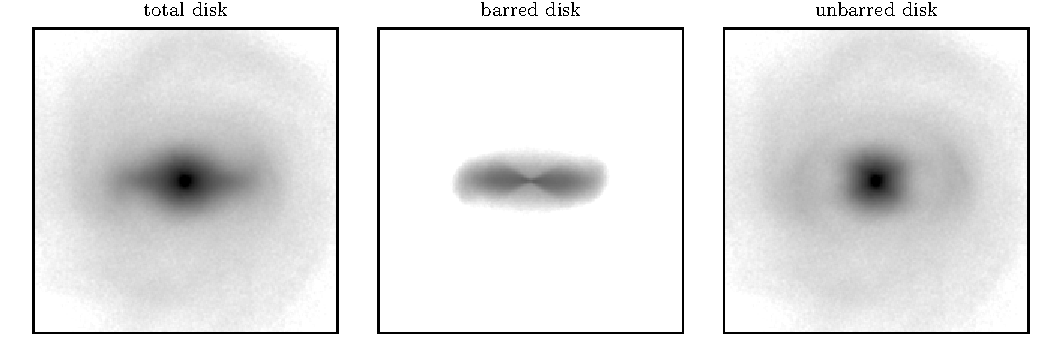
\includegraphics[width=\textwidth]{ch2/fig/bar_decomp.pdf}
    \caption{Disk decomposition into the barred and unbarred disk. This
    procedure is based on \citet{2016MNRAS.463.1952P}. The \textit{left panel}
    shows a face-on surface density projection through the stellar component of
    the \SMUGGLE{} simulation (disk and bulge) at $t=1\,\textrm{Gyr}$. The
    \textit{middle panel} shows the component of the disk identified as being
    trapped in the bar while the \textit{right panel} shows the component of the
    disk identified as not being trapped in the bar. The fact that the untrapped
    stars form a roughly axisymmetric structure indicates our bar decomposition
    is sufficiently accurate. We have computed that $76\%$ of the second Fourier
    component resides in the stars classified as being trapped in the bar.}
    \label{fig:decomp}
\end{figure*}

Computing the length of the bar and the torque on the bar by different
components requires us to decompose the disk into a component which is trapped
by the bar and a component which is untrapped. In order to do this, we follow
closely the technique developed in \citet{2016MNRAS.463.1952P}. We analyzed the
orbit of each star particle (meaning initial disk, bulge, and newly formed
stars) by extracting the $x$-$y$ positions of the apoapse of each in a frame
corotating with the bar, where apoapses are defined as local maxima in $r$. For
each apoapse, we searched for the $19$ closest apoapses in time and applied a
$k$-means clustering algorithm on this set of $20$ points with $k=2$. We then
computed for each of the two clusters the average angle from the bar
$\left<\Delta \phi\right>_{0,1}$, the standard deviation in $R$ of the points
${\sigma_R}_{0,1}$, and the average radius of the cluster
$\left<R\right>_{0,1}$. At each apoapse, a particle was considered to be in the
bar if it met the following criteria:
\begin{equation}
\textrm{max}\left(\left<\Delta \phi\right>_{0,1}\right) < \pi / 8
\end{equation}
\begin{equation}
\frac{{\sigma_R}_0 + {\sigma_R}_1}{\left<R\right>_0 + \left<R\right>_1} < 0.22
\end{equation}
These criterion are slightly different and simplified from the ones used in
\citet{2016MNRAS.463.1952P}, but we found them to empirically work well at
decomposing the disk into a bar and disk component. In Fig.~\ref{fig:decomp}, we
show an example of this decomposition. The \textit{left} panel shows a surface
density projection of the stellar disk and bulge (including newly formed stars)
from the \SMUGGLE{} model after $1\,\text{Gyr}$ of evolution in a frame such that
the bar is aligned with the $x$-axis. The \textit{middle} panel shows a
projection of the subset of stars that are identified as being trapped in the
bar and the \textit{right} panel shows a projection of the stars that are not
identified as being trapped. The fact that the \textit{right} panel is roughly
axisymmetric indicates the bar decomposition is performing adequately.

We computed the second Fourier component $A_2$ for all particles classified as
barred and unbarred. We found that $76\%$ of the total $m=2$ Fourier component
is in the particles classified as barred (i.e.,
$A_{2,\textrm{bar}}/A_{2,\textrm{tot}}\sim0.76$). Some of this is probably
coming from the $m=4$ component (e.g., boxy orbits) being classified as
unbarred, or the presence of weak spiral arms. See also
\citet{2021MNRAS.500..838P} for more details on the orbit family breakdown.

\section{Varying Pattern Speed}
\label{ch2:app:varyps}
When the bar slows down, we argue that this induces a larger positive torque
from the gas phase. Only gas within corotation will flow inwards, while gas
outside corotation will flow outwards \citep{2011MNRAS.415.1027H}. Since the
corotation radius is larger for more slowly rotating bars, it follows that
more slowly rotating bars should be more efficient at driving gas inflows and
thus experience a larger positive torque from the gas phase.

We performed an experiment to test this hypothesis by freezing the stellar
disk in the \SMUGGLE{} run and forcing it to rotate at a constant angular rate.
This has the effect of forcing the bar to rotate as a solid body at a constant
angular rate which we control. The gas is evolved self-consistently with this
rotating disk. We measured the torque on the bar by the gas phase at different
rotation rates. The result of this experiment is illustrated in
Fig.~\ref{fig:equil}, which shows that a more slowly rotating bar experiences a
larger positive torque from the gas.

We also note that since \citet{2011MNRAS.415.1027H} predicts gas outside of
corotation will flow outward, the bar should exert a positive torque on that
gas. Indeed, we measured the average torque on gas outside corotation from
$t=3\,\textrm{Gyr}$ to $5\,\textrm{Gyr}$ to be $0.87$ in code units
($10^{10}\,M_{\odot}\,(\text{km}/\text{s})^2$). For reference, the average
torque inside corotation is $-10.8$ over the same time period and in the same
units. So, while gas outside corotation does experience a positive torque, the
total torque on the gas phase is still negative.

\begin{figure*}
    \centering
    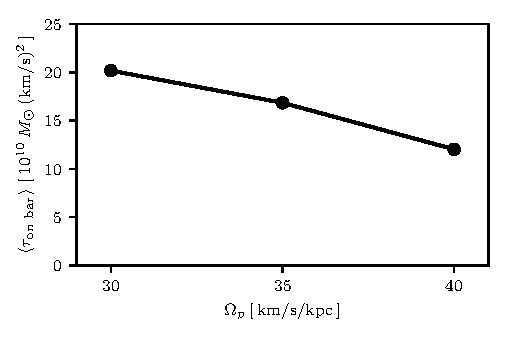
\includegraphics[width=9cm]{ch2/fig/torque_ps.pdf}
    \caption{Average torque exerted by gas on a bar which rotates at a fixed
    pattern speed. Since only gas within the corotation radius is able to infall
    and slower bars have larger corotation radii, slower bars experience a
    larger net torque than faster bars. The setup of the simulations used here
    is identical to the \SMUGGLE{} case discussed earlier, except the \Nbody{} disk
    is rotated as a solid body with a constant angular
    velocity.}
    \label{fig:equil}
\end{figure*}

\begin{figure*}
    \centering
    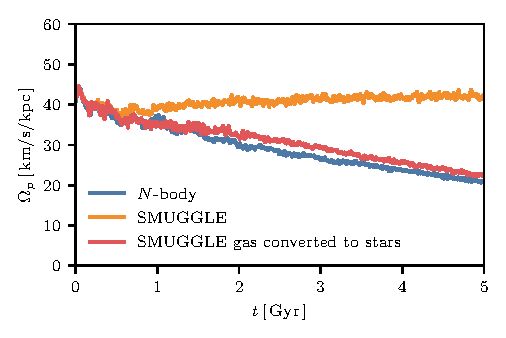
\includegraphics[width=9cm]{ch2/fig/ps_star.pdf}
    \caption{Pattern speed evolution of a model in which we instaneously
    add stars instead of gas to the simulation, with the same density profile as
    the gas phase. The pattern speed evolution in this case is qualitatively
    similar to that of the $N$-body case, with a slight offset in the pattern
    speed. This test demonstrates that the stable pattern speed evolution in the
    SMUGGLE case is not simply a consequence of the change in potential imposed
    in our initial conditions.}
\label{fig:ps-star}
\end{figure*}

\section{Stars Instead of Gas}
In the SMUGGLE model considered in this work, we instantaneously added gas to
the $N$-body system after $1.5\,\textrm{Gyr}$ of evolution. One might wonder if
this sudden change to the potential is responsible for the stable pattern speed
evolution. To test whether this is the case, we added mass to the system in the
same way we did for the SMUGGLE model, but using collisionless particles instead
of gas. The result of this experiment is shown in Fig.~\ref{fig:ps-star}. While
there is an offset compared to the pure $N$-body case, we see that the pattern
speed evolution is broadly consistent with a declining pattern speed. This
indicates that the gas phase is responsible for the stable pattern speed.

\begin{figure}
    \centering
    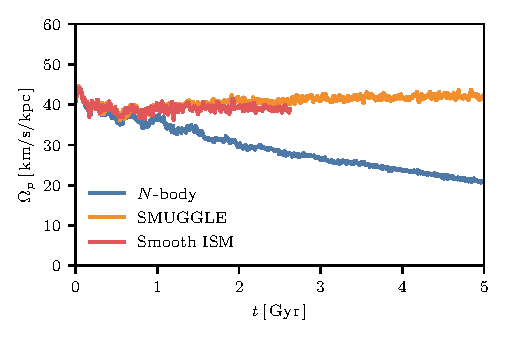
\includegraphics[width=9cm]{ch2/fig/ps_GFM.pdf}
    \caption{Pattern speed evolution of a smooth ISM model. This evolution is
    shown for the fiducial disk in the \Nbody{} (blue), \SMUGGLE{} (orange), and
    smooth ISM (red) cases. The smooth ISM model is an older model for the ISM
    which treats its multiphase nature in a subgrid fashion
    \citep{2003MNRAS.339..289S}. This fundamentally differs from the \SMUGGLE{}
    model, which explicitly resolves the hot and cold phases of the ISM
    \citep{2019MNRAS.489.4233M}. The pattern speed in the smooth ISM case is
    broadly similar to the evolution in the \SMUGGLE{} case. This shows that the
    stability of the pattern speed is not simply a result of our assumed model
    for the ISM.}
\label{fig:GFM}
\end{figure}

\section{Smooth Interstellar Medium}
We performed a simulation of the same disk but with a simpler model of the
interstellar medium \citep{2003MNRAS.339..289S}, closer to standard methods used
in cosmological simulations of galaxy formation and described in more detail in
Section~\ref{ch2:sec:methods}. The result of this test is presented in
Fig.~\ref{fig:GFM}. We find that the pattern speed evolution is nearly the same
in this case, and so conclude that our result is not sensitive to the details of
the model for the interstellar medium.

\section{Semi-Analytic Model Parameters}
\label{ch2:app:sam}
Our semi-analytic model consisted of a three-component bar-disk-halo system. We
describe here the parameters we chose for these components. The parameters of
the disk and halo were chosen to match closely what we used in our fiducial
simulations. The system can thus be understood as being roughly similar to the
Milky Way, though no careful analysis has been performed to ensure the closest
match possible.

For the dark matter halo, we used a Hernquist potential
\citep{1990ApJ...356..359H} with mass $10^{12}\,\Msun$ and a scale length of
$26.2\,\textrm{kpc}$. For the stellar disk, we used a Miyamoto-Nagai disk
\citep{1975PASJ...27..533M} with mass $4.8\times10^{10}\,\Msun$, radial scale
length of $2.67\,\textrm{kpc}$, and vertical scale length of
$0.32\,\textrm{kpc}$. For the bar, we used the quadrupole potential described in
\citet{2022MNRAS.513..768C}. We used their fiducial parameter values --
specifically, we set $A=0.02$, $b=0.28$, and $v_c = 235\,\kms$. Our initial
pattern speed is always set to $40\,\kms/\textrm{kpc}$.

We integrated our model for $5\,\textrm{Gyr}$ with a timestep of
$0.01\,\textrm{Gyr}$.

\section{Comparison to the Milky Way}
\label{ch2:app:milkyway}
For several Gyr, our fiducial disk exhibits several properties in reasonable
agreement to the Milky Way. This is uncommon in models of galaxies that include
the gas phase of the disk but no circumgalactic medium. As mentioned earlier,
the pattern speed seems to match the observed pattern speed of the Milky Way's
bar \citep{2019MNRAS.490.4740B}. We briefly summarize some of the other ways our
disk is comparable to the Milky Way.

We computed the circular velocity curve of our model using the \texttt{AGAMA}
package \citep{2019MNRAS.482.1525V}. We fit the baryonic component (stellar
disk, bulge, gas, and newly formed stars) with an axisymmetric cylindrical
spline with $20$ grid points in both the radial and vertical direction spanning
$0.2$ to $50\,\textrm{kpc}$ in the radial direction and from $0.02$ to
$10\,\textrm{kpc}$ in the vertical direction. We fit the dark matter halo using
an axisymmetric multipole fit with a maximum angular harmonic coefficient
of $l=2$, to account for the compression of the halo by the disk. We plot
the circular velocity curve at $t=1\,\textrm{Gyr}$ in Fig.~\ref{fig:vcirc}
compared to observational estimates \citep{2019ApJ...871..120E}. The \SMUGGLE{}
disk (which includes additional mass in the form of gas) has a slightly higher
circular velocity than the \Nbody{} disk which, itself, is slightly higher than
the observational estimates. Overall, though, the circular velocity curves
between our model and that observed in the Milky Way are broadly consistent.

We also show the evolution of the surface density profile in Fig.~\ref{fig:surf}
We find that in our simulation the atomic and molecular gas surface density and
the SFR surface density is broadly consistent with the expected values for the
Milky Way \citep{2008A&A...487..951K,2022ApJ...929L..18E}. The discrepancy between
$1$ and $4\,\textrm{kpc}$ in the molecular and SFR surface density is probably due
to the fact that the distances to molecular clouds which underlines this work
used a simple kinematic distance based on an axisymmetric model of the Milky
Way \citep{2017ApJ...834...57M}, which is not accurate in the bar region where gas
has large non-circular velocities.

We measured the initial scale height of the atomic gas disk in a bin
extending from $R=7.5\,\textrm{kpc}$ to $R=8.5\,\textrm{kpc}$. The initial
vertical profile is well-fit by a Gaussian with a scale height of
$110\,\textrm{pc}$. At $t=1\,\textrm{Gyr}$, the vertical profile in the same
radial bin is better fit by an exponential profile with scale height of
$74\,\textrm{pc}$. These are somewhat lower than the observed value in the HI
disk of $\sim200\,\textrm{pc}$ \citep{1995ApJ...448..138M, 2017A&A...607A.106M}.
This may be caused by the model in our simulations not driving enough turbulent
pressure, and is an interesting avenue of further investigation.

\begin{figure*}
    \centering
    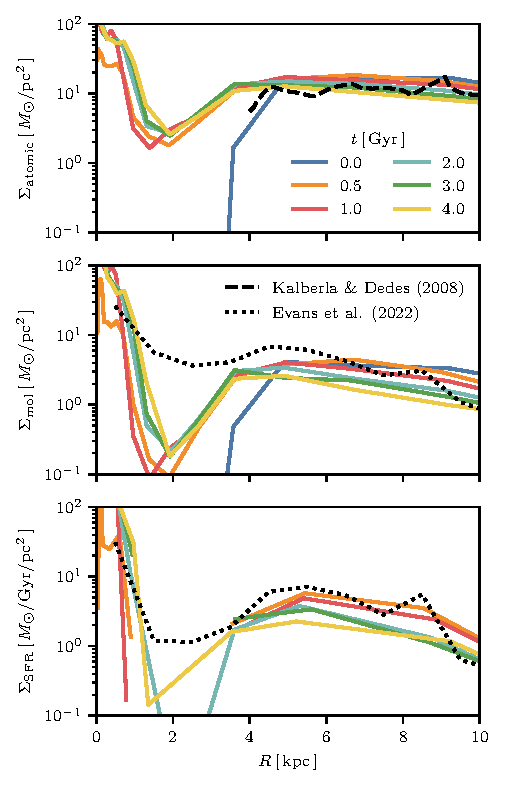
\includegraphics[width=9cm]{ch2/fig/surf_dens.pdf}
    \caption{The time evolution of the atomic gas surface density
    (\textit{upper}), molecular gas surface density (\textit{middle}) and the
    star formation rate (SFR) surface density (\textit{lower}) at various times
    during our fiducial simulation. Colored lines indicate the profiles at
    selected times during the simulation while the black dashed lines indicate
    observations for the atomic gas \citep{2008A&A...487..951K} and black dotted
    lines indicate a model which allows the CO-to-H$_2$ conversion factor
    $X_{\textrm{CO}}$ to vary with metallicity \citep{2022ApJ...929L..18E}.
    Molecular gas surface densities were provided separately (N. Evans, private
    communication). We see that the molecular gas and SFR surface densities are
    within an order of magnitude of the Milky Way's typical values at all times.
    We see a sharp decrease in the gas and SFR surface densities along the
    extent of the bar from $\sim1$ to $\sim4\,\textrm{kpc}$, related to the gas
    inflow in this region.}
    \label{fig:surf}
\end{figure*}

\begin{figure}
    \centering
    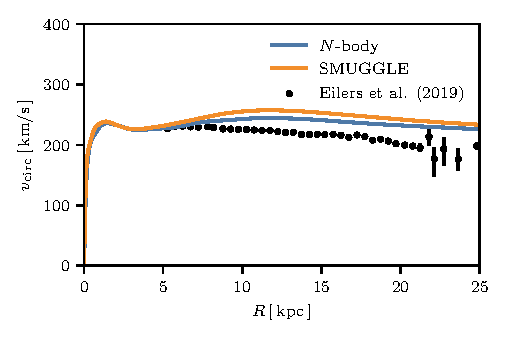
\includegraphics[width=9cm]{ch2/fig/vcirc.pdf}
    \caption{The circular velocity curve of our setups at $t=1\,\textrm{Gyr}$.
    This curve is shown for the \Nbody{} run (blue) and the \SMUGGLE{} run
    (orange) compared to observational estimates for the Milky Way
    \citep{2019ApJ...871..120E}. We see that the circular velocity curve for
    both runs is marginally larger than the Milky Way's, but still comparable.
    The \SMUGGLE{} circular velocity curve is larger than the \Nbody{} curve due
    to the additional mass in the gas phase.}
    \label{fig:vcirc}
\end{figure}

\chapter{Appendix to Chapter~\ref{ch:GSEgas}}\label{ch:app_GSEgas}

\section{Star Formation Histories}\label{ch3:app:all_sfh}
One potential avenue for creating an \FeH{}-dependent star formation gap is through quiescence. This is demonstrated by examining the global SFH in Figure~\ref{fig:all_sfh}, with the panels and colors showing each simulation in the grid ordered by their bimodality score $\mathcal{B}$ in the same way as Figures~\ref{ch3:fig:all_hist} and \ref{ch3:fig:all_scatter}. One can see that there is a global quiescent period in simulations~g, s, and x. Simulations~s and x have a bimodal pattern, while simulation~g has a unimodal pattern. As mentioned in Figure~\ref{ch3:fig:all_scatter}, simulation~g has an age gap but there is not enough star formation at $\FeH\sim0$ before the gap to result in a strong bimodality. Otherwise, while a global quiescent period is sufficient for generating an age gap, most simulations do not have a global quiescent period.

\begin{figure*}
  \centering
  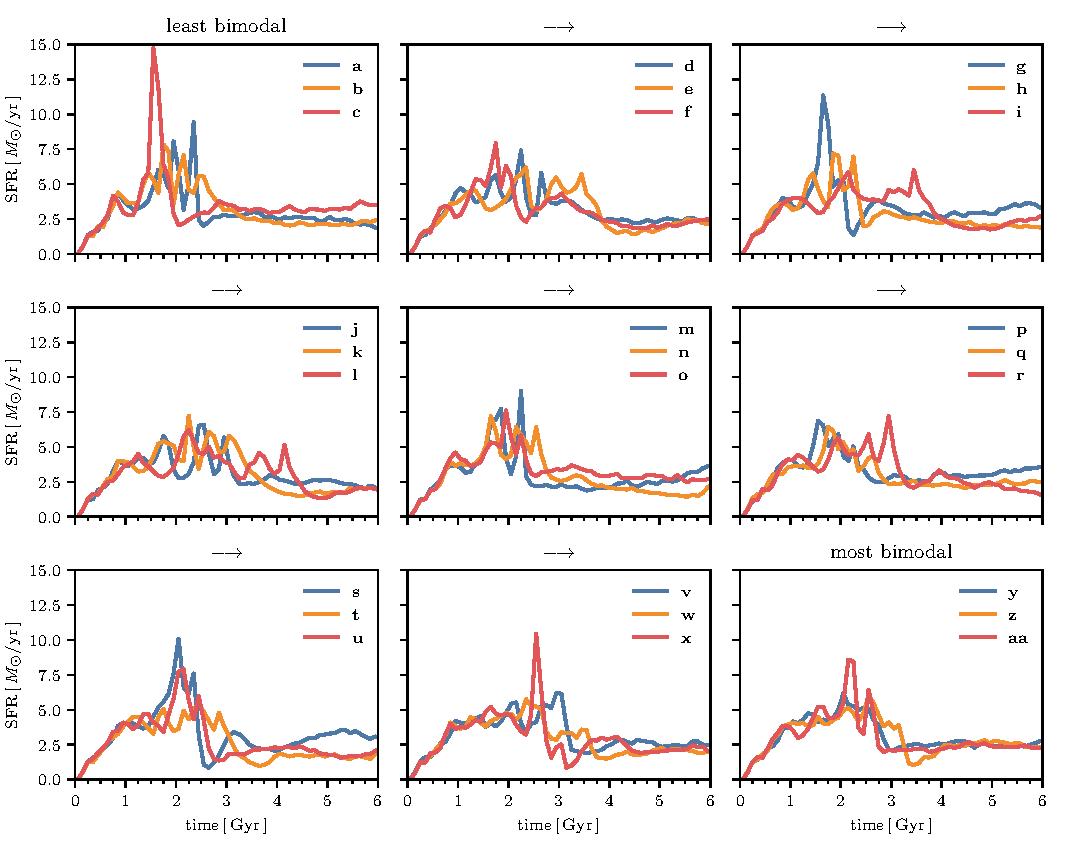
\includegraphics[width=\textwidth]{ch3/sfh.pdf}
  \caption{Global star formation history (SFH) for each simulation, plotted in the same order as Figures~\ref{ch3:fig:all_hist} and \ref{ch3:fig:all_scatter}, with increasing bimodality score $\mathcal{B}$ from left to right. The colors correspond to the same simulations as in previous figures. A global quiescent period, characterized by a significant dip in the SFR, is observed in simulations~g, s, and x. Among these, simulations~s and x exhibit strong bimodal \MgFe{} distributions, while simulation~g remains unimodal due to insufficient early star formation at $\FeH\sim0$ before the quiescent phase. Most other simulations do not display a clear global quiescent period, indicating that such a phase is not strictly necessary for bimodality to emerge.}
  \label{fig:all_sfh}
\end{figure*}

\section{Cause of Suppressed Star Formation}\label{ch3:app:cause_qui}
In Figure~\ref{fig:MdotBH_rsep}, we demonstrate how the orbit of the bimodal simulation is closely related to the strength of BH feedback. On the $y$-axis, we show in blue the black hole accretion rate as a ratio of the maximum (Eddington) accretion rate at that time. In orange we show the orbital separation between the satellite and central galaxies. We see that the accretion rate is high early on at $\sim10\%$. At the time around coalescence at $\sim2\,\Gyr$, the accretion rate rises up to Eddington, before dropping to a much lower value $<10\%$ later on.

In the TNG model, the strength of AGN feedback is directly tied to the BH's accretion rate \citep{2017MNRAS.465.3291W}. Therefore, it is reasonable to suspect that the feedback from the AGN is responsible for removing gas from the galaxy or keeping it above the star forming density threshold.

\begin{figure}
  \centering
  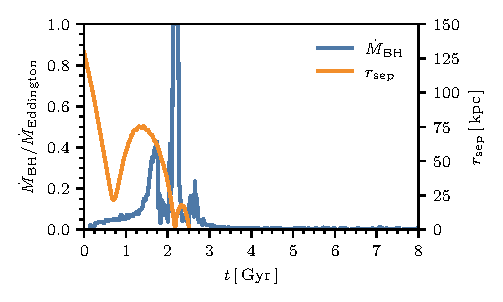
\includegraphics[width=242.26653pt]{ch3/MdotBH_rsep.pdf}
  \caption{Evolution of black hole accretion rate and orbital separation over time in the bimodal simulation. The blue line shows the black hole accretion rate as a fraction of the Eddington rate, while the orange line shows the orbital separation between the satellite and central galaxies. The accretion rate peaks during coalescence at $\sim2\,\Gyr$, suggesting a strong connection between the merger and AGN activity.}
  \label{fig:MdotBH_rsep}
\end{figure}

\section{Abundance Plane of All Simulations}\label{ch3:app:allmerge}
We show summary plots of the abundance planes of all simulations in our orbital grid in Figures~\ref{fig:allmerge0} to \ref{fig:allmerge8}.

\begin{figure*}
  \centering
  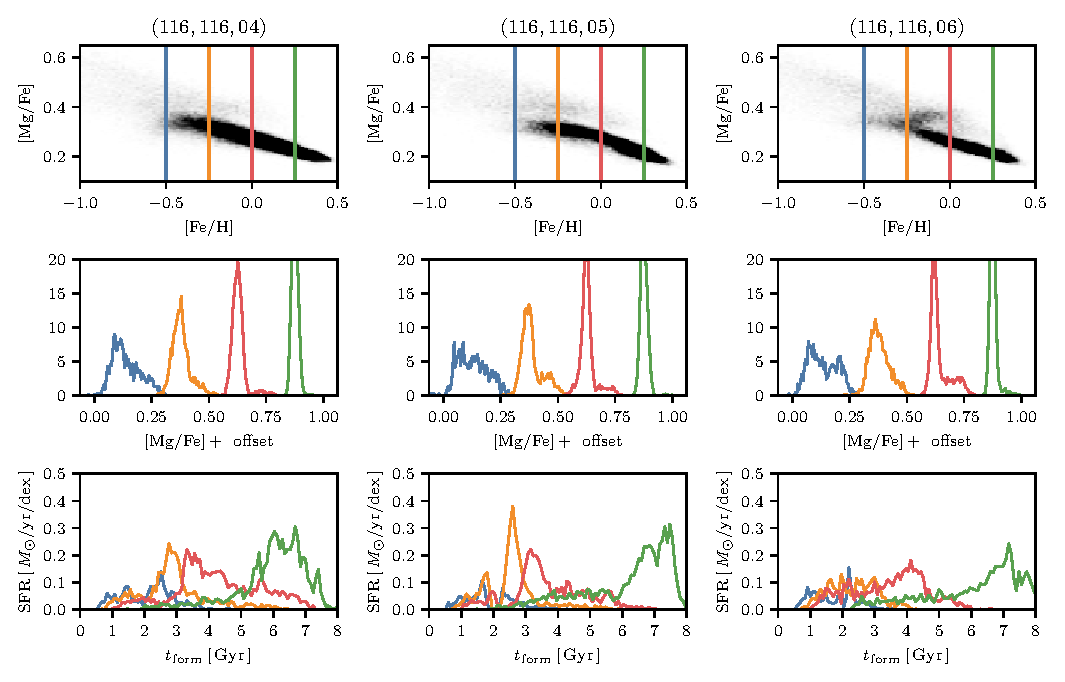
\includegraphics[width=\textwidth]{ch3/allmerge0.pdf}
  \caption{A summary of the abundance plane and star formation history of all simulations within the orbital grid. Each figure shows the outcome of a simulation at a fixed $R_0$ and $V_0$, varying $\eta$. The title of each column shows the $R_0$, $V_0$, and $\eta$ of that simulation, in order. The upper and middle rows replicate Figure~\ref{ch3:fig:fig1}, which show the distribution of stars in the abundance plane of \MgFe{}-\FeH{} as well as 1D histograms at a fixed \FeH{} of $-0.5$, $-0.25$, $0$, and $0.25$. The lower rows replicate Figure~\ref{ch3:fig:before_after_sfh_by_iron}, showing the star formation history at each \FeH{}.}
  \label{fig:allmerge0}
\end{figure*}

\begin{figure*}
  \centering
  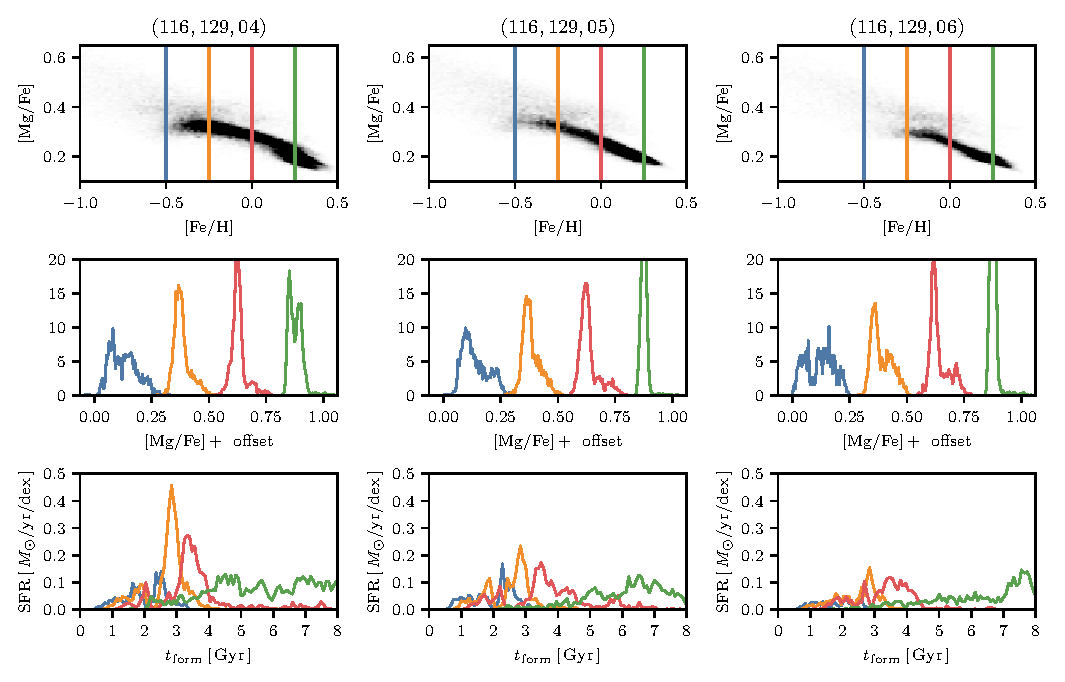
\includegraphics[width=\textwidth]{ch3/allmerge1.pdf}
  \caption{A continuation of Figure~\ref{fig:allmerge0}.}
  \label{fig:allmerge1}
\end{figure*}

\begin{figure*}
  \centering
  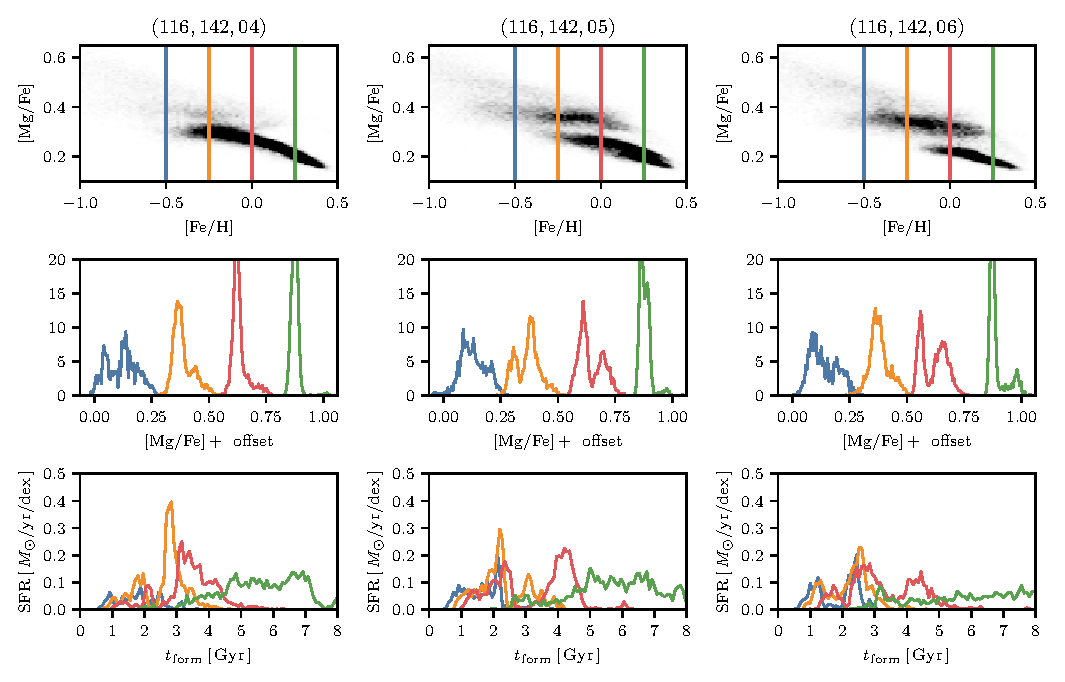
\includegraphics[width=\textwidth]{ch3/allmerge2.pdf}
  \caption{A continuation of Figure~\ref{fig:allmerge0}.}
  \label{fig:allmerge2}
\end{figure*}

\begin{figure*}
  \centering
  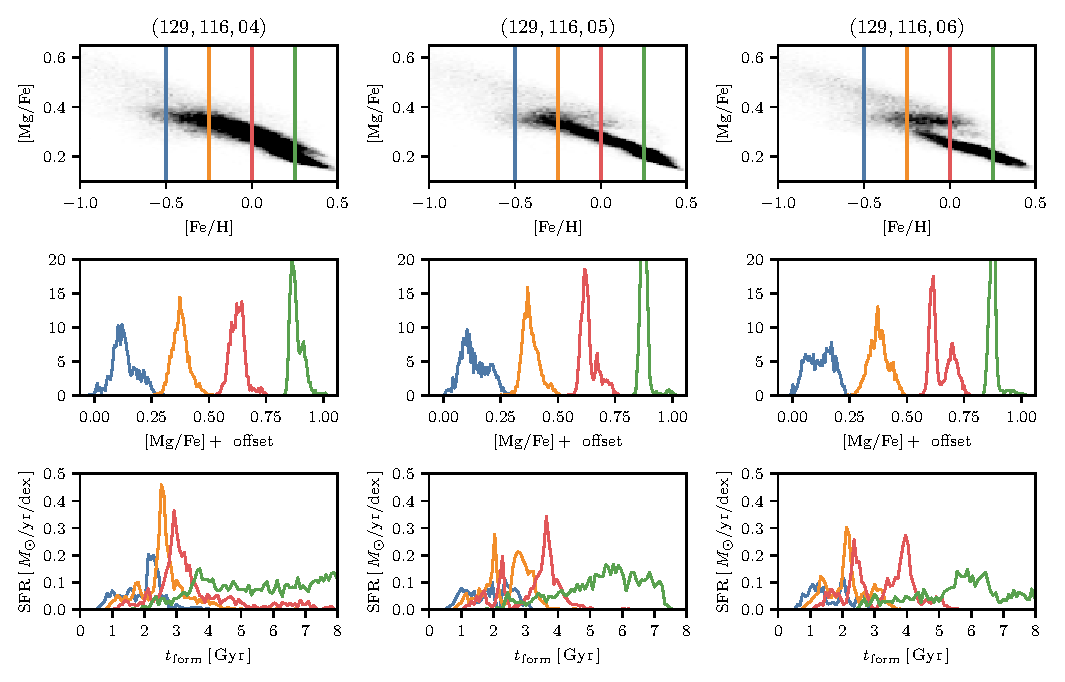
\includegraphics[width=\textwidth]{ch3/allmerge3.pdf}
  \caption{A continuation of Figure~\ref{fig:allmerge0}.}
  \label{fig:allmerge3}
\end{figure*}

\begin{figure*}
  \centering
  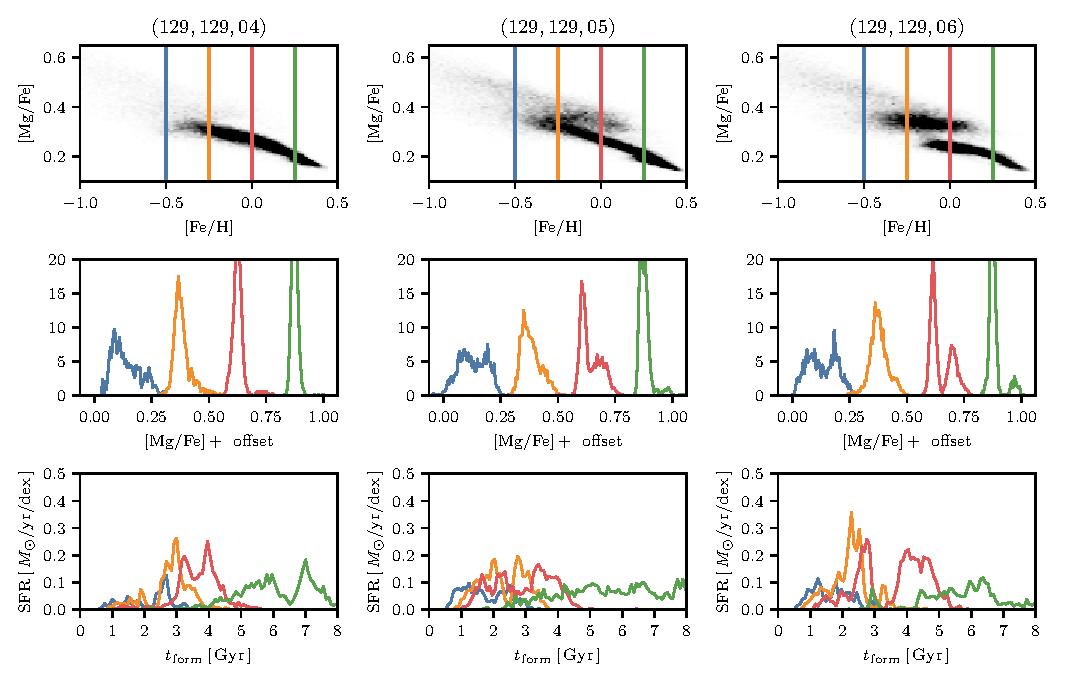
\includegraphics[width=\textwidth]{ch3/allmerge4.pdf}
  \caption{A continuation of Figure~\ref{fig:allmerge0}.}
  \label{fig:allmerge4}
\end{figure*}

\begin{figure*}
  \centering
  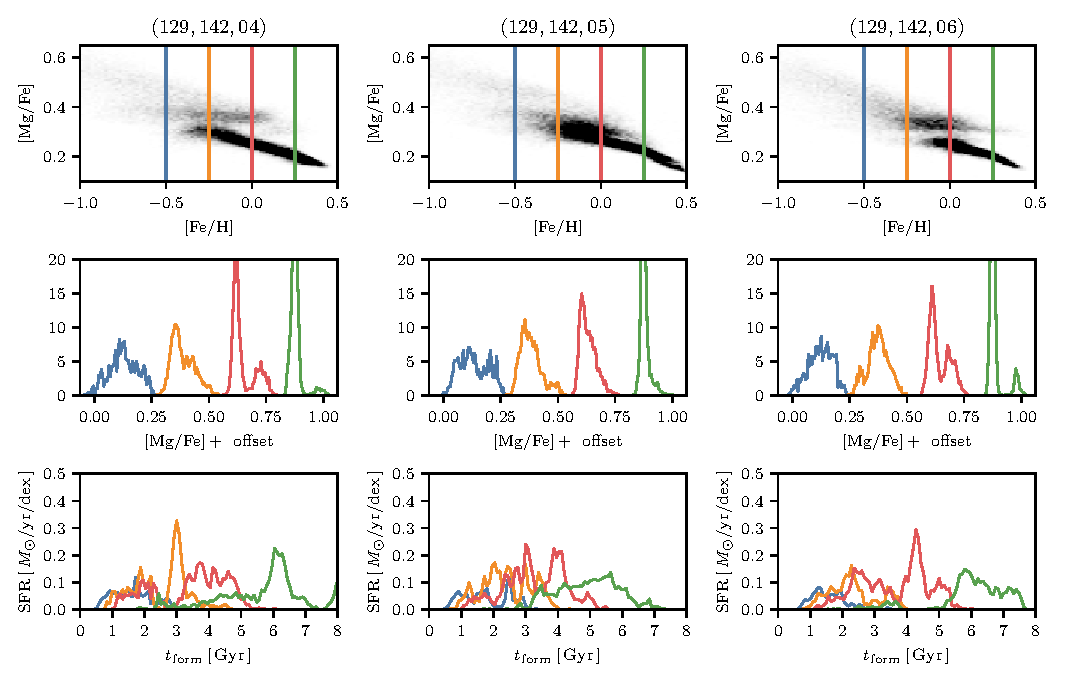
\includegraphics[width=\textwidth]{ch3/allmerge5.pdf}
  \caption{A continuation of Figure~\ref{fig:allmerge0}.}
  \label{fig:allmerge5}
\end{figure*}

\begin{figure*}
  \centering
  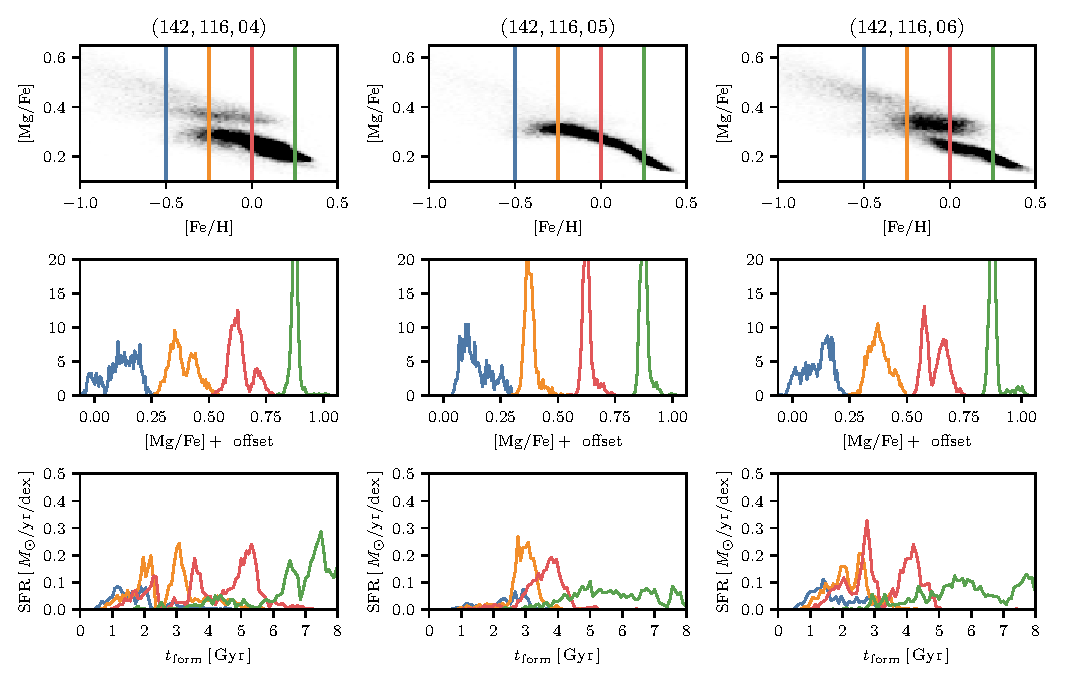
\includegraphics[width=\textwidth]{ch3/allmerge6.pdf}
  \caption{A continuation of Figure~\ref{fig:allmerge0}.}
  \label{fig:allmerge6}
\end{figure*}

\begin{figure*}
  \centering
  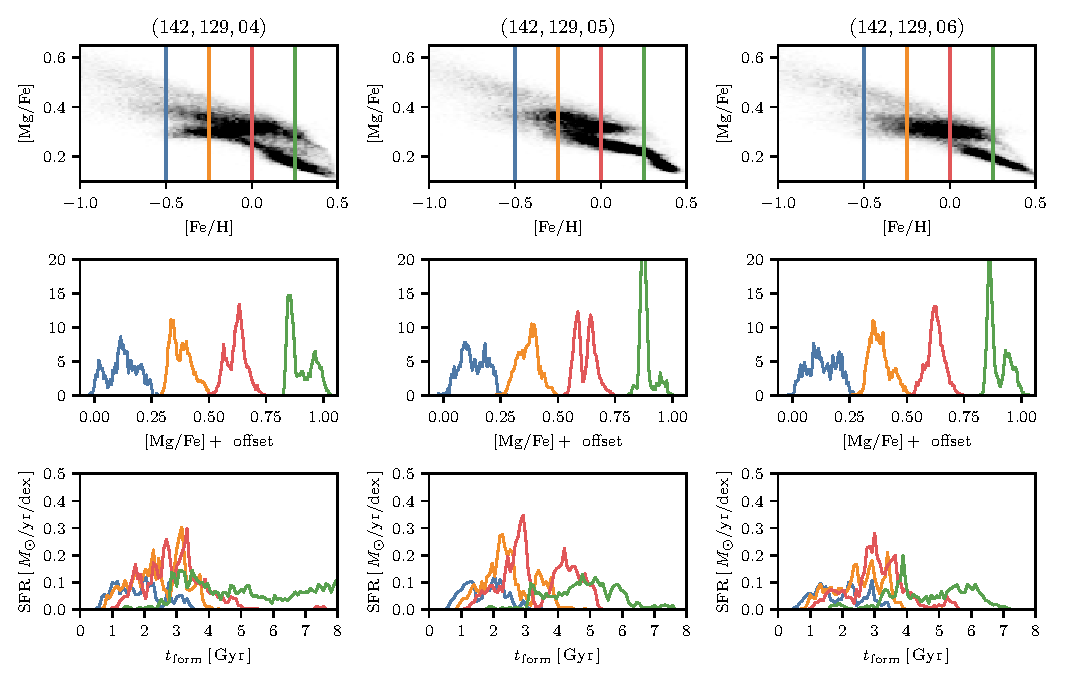
\includegraphics[width=\textwidth]{ch3/allmerge7.pdf}
  \caption{A continuation of Figure~\ref{fig:allmerge0}.}
  \label{fig:allmerge7}
\end{figure*}

\begin{figure*}
  \centering
  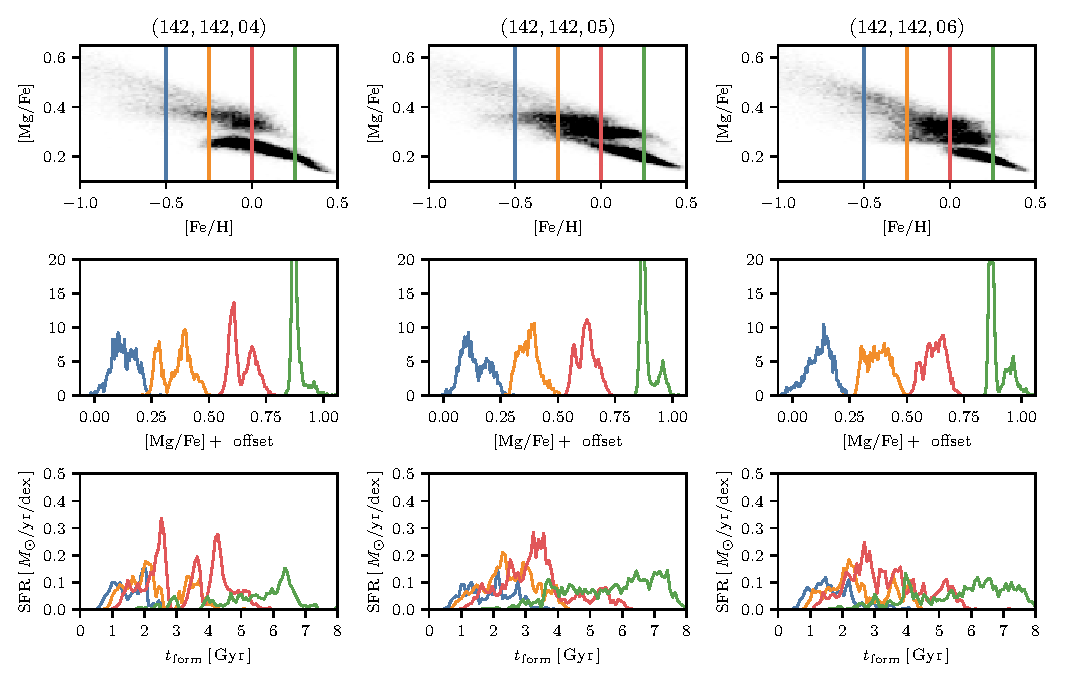
\includegraphics[width=\textwidth]{ch3/allmerge8.pdf}
  \caption{A continuation of Figure~\ref{fig:allmerge0}.}
  \label{fig:allmerge8}
\end{figure*}

\chapter{Appendix to Chapter~\ref{ch:Mgdec}}\label{ch:app_Mgdec}
\section{Observational Errors}\label{ch4:app:obs_err}
In Figure~\ref{fig:alpha}, we assumed observational errors of $12.5\%$ in age and $0.015\,\dex$ in \MgFe{}. In Figure~\ref{fig:obs_err}, we plot the quoted observational errors of the APOKASC-3 (left) and ASPCAP (right) datasets, showing both \FeH{} and \MgFe{} (blue and orange, respectively). We show our $12.5\%$ age error as a black line in the left panel. We take the age error to be the maximum of the upper and lower errors from \citet{2018ApJS..239...32P}. In the right panel, we show blue and orange vertical lines at $0.01$ and $0.015\,\dex$ for \FeH{} and \MgFe{}, respectively. These are approximately the 99th percentiles of each error distribution. As a dashed line we show our $25\%$ age error cut for stars plotted in Figure~\ref{fig:obs_err}. Our assumed errors are generally consistent with the errors quoted in the dataset, with a conservative estimate for the abundance errors.

\begin{figure*}
  \centering
  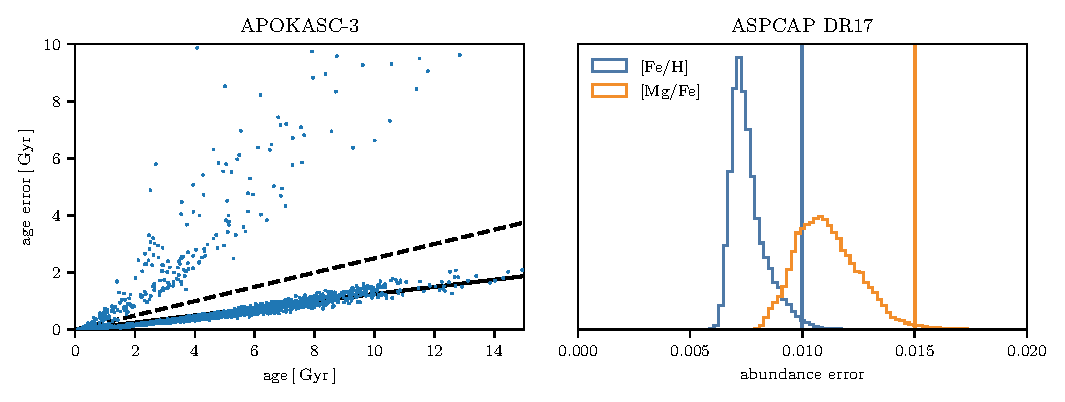
\includegraphics[width=\columnwidth]{ch4/obs_error.pdf}
  \caption{The observational errors of astroseismic ages from APOKASC-3 (left) and abundances from ASPCAP DR17 (right). We show, on the left, a line indicating a $12.5\%$ error in observed age and on the right a vertical line indicating a $0.01$ and $0.015\,\dex$ error in \FeH{} and \MgFe{}, respectively. On the left, a dashed line indicates the $25\%$ error cut used for inclusion in Figure~\ref{fig:alpha}.}
  \label{fig:obs_err}
\end{figure*}

\section{Random Selection of Subhalos}\label{ch4:app:rand_fig1}
In Figure~\ref{fig:app0}, we show the abundance plane of our fiducial galaxy at $z=0$. This reproduces the middle column of Figure~\ref{fig:fig1}. We also show the effect of our $\alpha$-enhancement procedure on this distribution when applied, from left to right, at redshifts of $1$, $1.5$, and $2$. (The $z=1.5$ column reproduces the right column of Figure~\ref{fig:fig1}). Qualitatively, the time at which the $\alpha$-enhancement is applied does not alter whether substructure arises in this plane. However, when it is applied at lower $z$, the peaks between modes do appear to be slightly further apart.

We show the same figure but with an additional random selection of 16 galaxies in the Milky Way-progenitor mass sample as a figure set (17 images), which is available in the online journal. Six additional galaxies (143882, 167392, 348901, 425719, 439099, and 465255) display bimodalities, though none as prominent as the main galaxy studied in this work. Some substructure is present in many galaxies. In general, the $\alpha$-enhancement increases the strength of substructure in the abundance planes. The fact that bimodalities like in the main galaxy studied in this work do not universally appear in $\alpha$-enhanced galaxies indicates that the $\alpha$-enhancement is not solely responsible for the bimodality.

The timing of the $\alpha$-enhancement does not have a major effect on our fiducial galaxy (Figure~\ref{fig:app0}). However, for some (e.g., the green $\FeH=-0.25$ bin in 439099), structure arises only when the $\alpha$-enhancement is applied at sufficiently low redshift. We interpret this as the presence of some substructure inducing activity between $z=1$ and 2.

\begin{figure*}
  \centering
  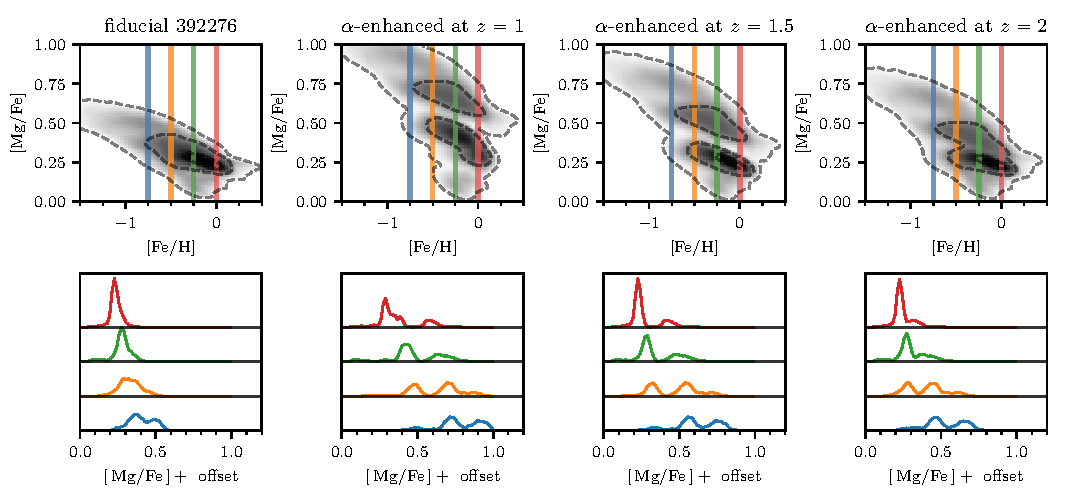
\includegraphics[width=\textwidth]{ch4/app_392276.pdf}
  \caption{Abundance plane of the fiducial galaxy at $z=0$ and the effects of $\alpha$-enhancement applied at different redshifts. The leftmost panel shows the fiducial galaxy without enhancement, reproducing the middle column of Figure~\ref{fig:fig1}. The subsequent panels from left to right show the results of applying $\alpha$-enhancement at redshifts of 1, 1.5, and 2, respectively. The $z=1.5$ column reproduces the right column of Figure~\ref{fig:fig1}. The presence of substructure in the abundance plane is consistent across different application times of $\alpha$-enhancement, though applying it at lower redshifts appears to slightly increase the separation between modal peaks. This figure is part of a set of 17 images available in the online journal, showing similar plots for 16 additional galaxies from our Milky Way-progenitor mass sample. The varied responses to $\alpha$-enhancement across the sample, with only six additional galaxies (143882, 167392, 348901, 425719, 439099, and 465255) displaying bimodalities, suggest that while $\alpha$-enhancement generally increases substructure, it is not solely responsible for creating bimodalities in abundance planes.}
  \label{fig:app0}
\end{figure*}

\begin{figure*}
  \centering
  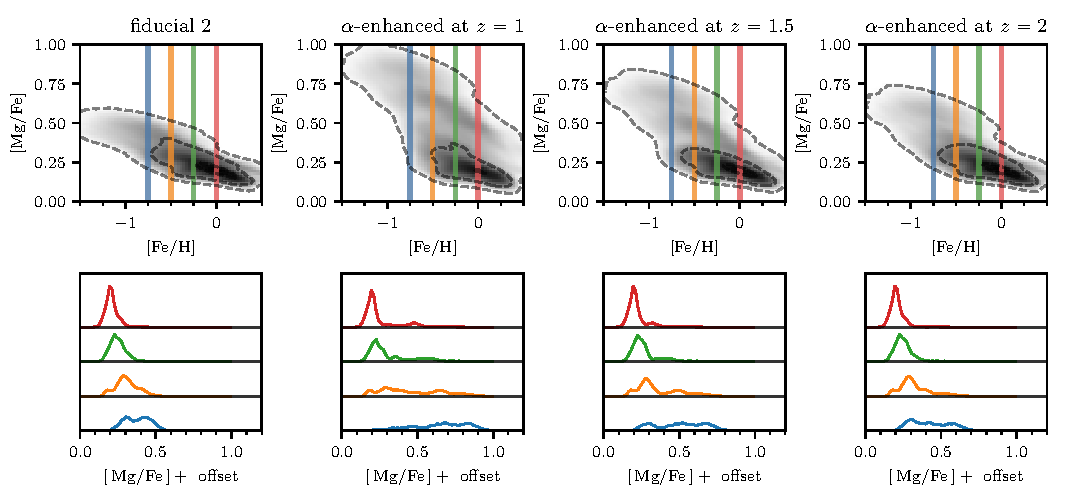
\includegraphics[width=\textwidth]{ch4/app_2.pdf}
  \caption{The same as Figure~\ref{fig:app0}, but for a random galaxy from our initial catalog.}
  \label{fig:app1}
\end{figure*}

\begin{figure*}
  \centering
  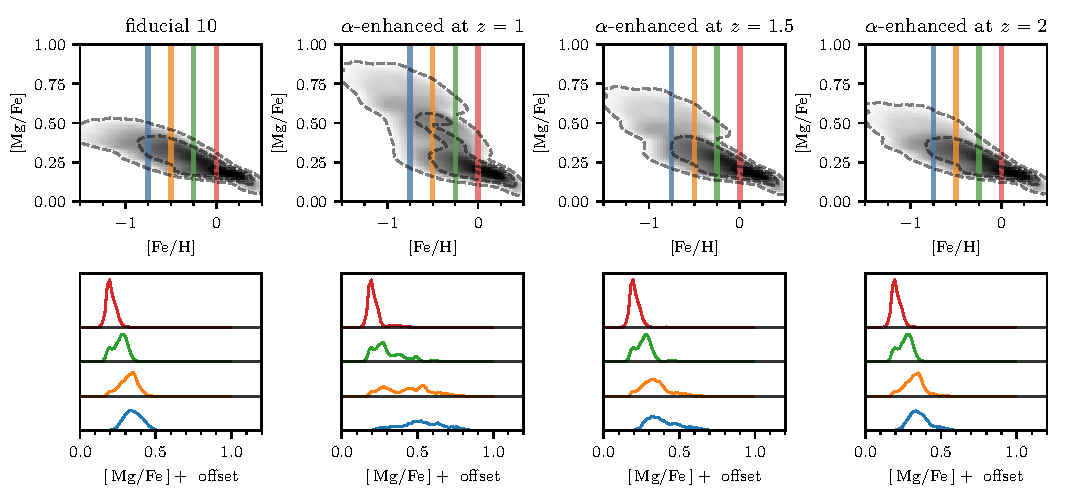
\includegraphics[width=\textwidth]{ch4/app_10.pdf}
  \caption{The same as Figure~\ref{fig:app0}, but for a random galaxy from our initial catalog.}
  \label{fig:app2}
\end{figure*}

\begin{figure*}
  \centering
  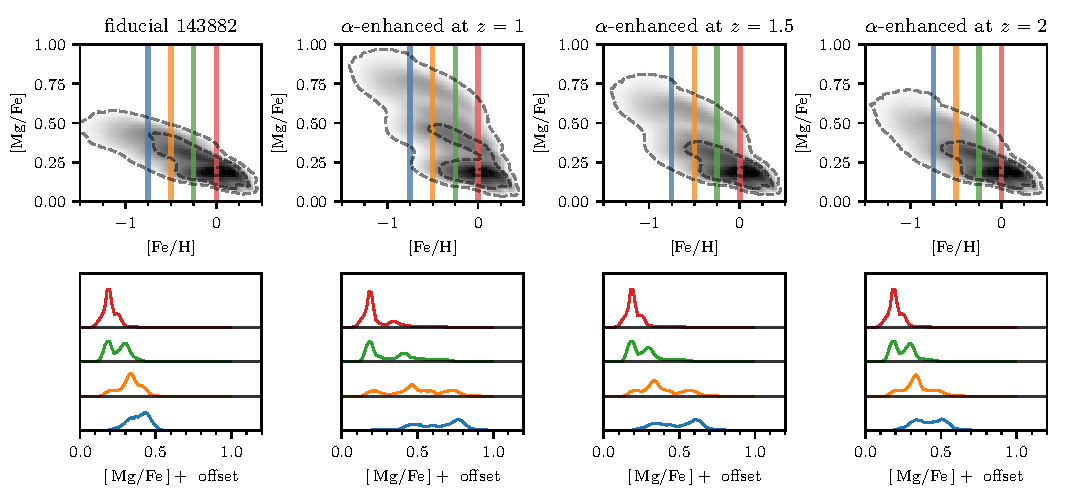
\includegraphics[width=\textwidth]{ch4/app_143882.pdf}
  \caption{The same as Figure~\ref{fig:app0}, but for a random galaxy from our initial catalog.}
  \label{fig:app3}
\end{figure*}

\begin{figure*}
  \centering
  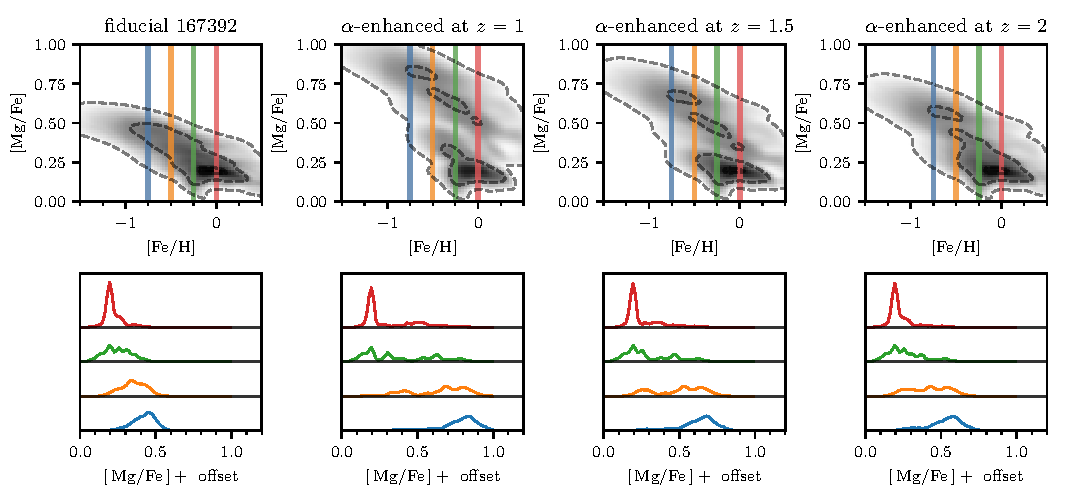
\includegraphics[width=\textwidth]{ch4/app_167392.pdf}
  \caption{The same as Figure~\ref{fig:app0}, but for a random galaxy from our initial catalog.}
  \label{fig:app4}
\end{figure*}

\begin{figure*}
  \centering
  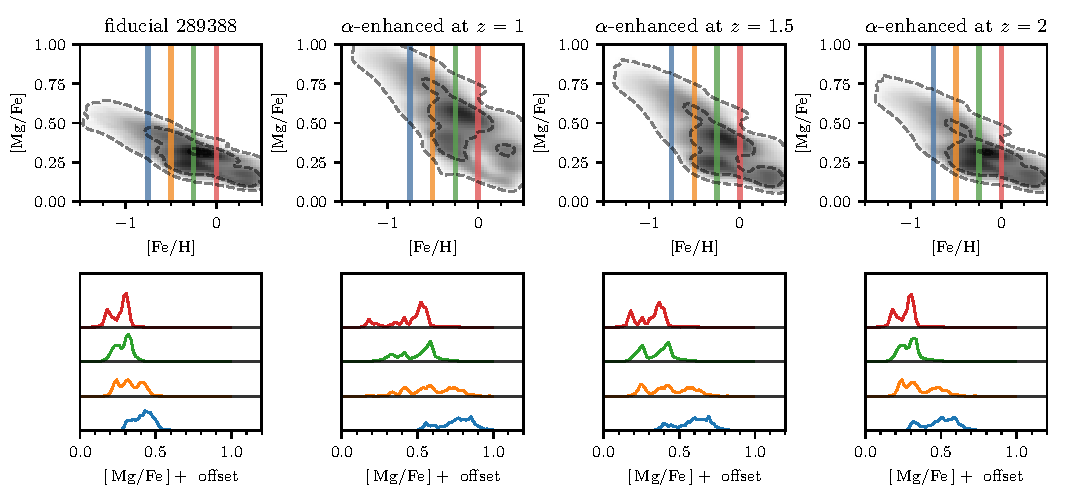
\includegraphics[width=\textwidth]{ch4/app_289388.pdf}
  \caption{The same as Figure~\ref{fig:app0}, but for a random galaxy from our initial catalog.}
  \label{fig:app5}
\end{figure*}

\begin{figure*}
  \centering
  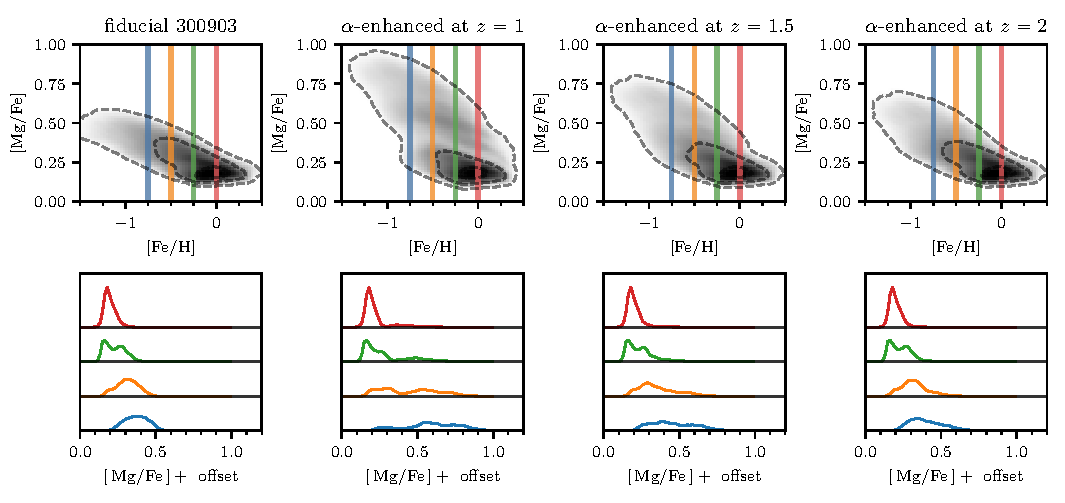
\includegraphics[width=\textwidth]{ch4/app_300903.pdf}
  \caption{The same as Figure~\ref{fig:app0}, but for a random galaxy from our initial catalog.}
  \label{fig:app6}
\end{figure*}

\begin{figure*}
  \centering
  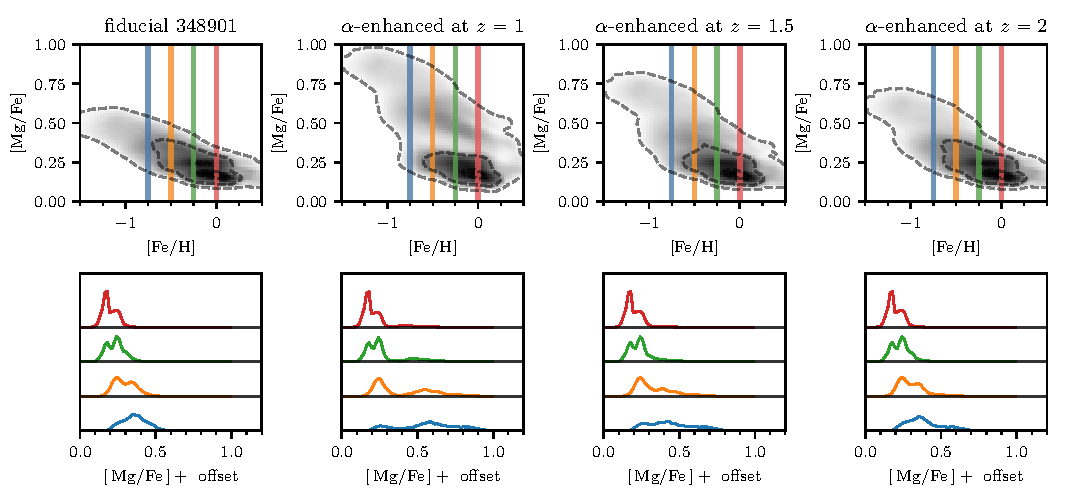
\includegraphics[width=\textwidth]{ch4/app_348901.pdf}
  \caption{The same as Figure~\ref{fig:app0}, but for a random galaxy from our initial catalog.}
  \label{fig:app7}
\end{figure*}

\begin{figure*}
  \centering
  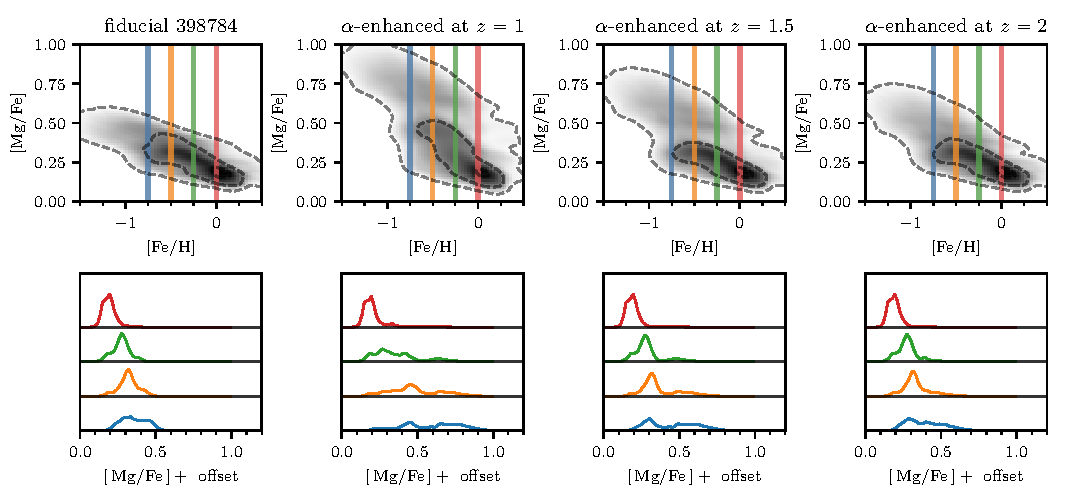
\includegraphics[width=\textwidth]{ch4/app_398784.pdf}
  \caption{The same as Figure~\ref{fig:app0}, but for a random galaxy from our initial catalog.}
  \label{fig:app8}
\end{figure*}

\begin{figure*}
  \centering
  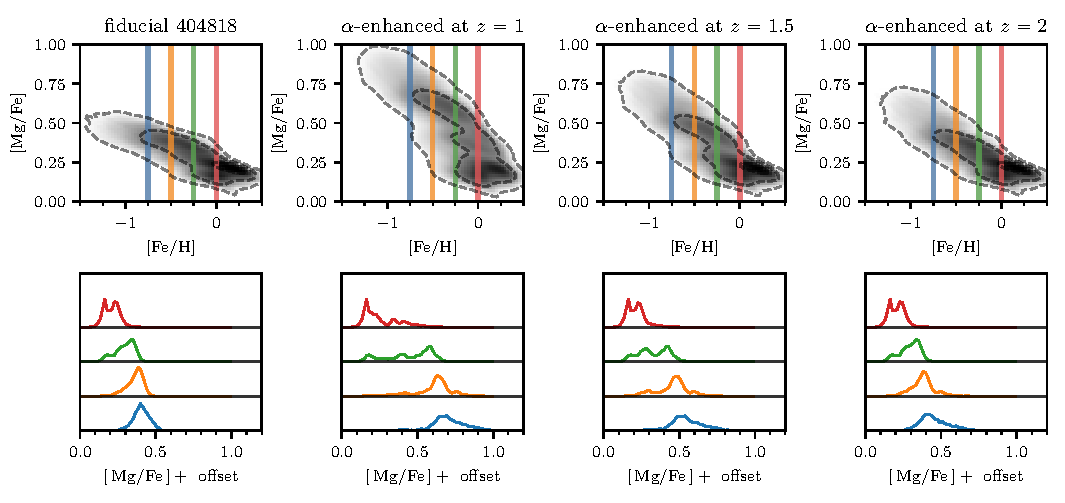
\includegraphics[width=\textwidth]{ch4/app_404818.pdf}
  \caption{The same as Figure~\ref{fig:app0}, but for a random galaxy from our initial catalog.}
  \label{fig:app9}
\end{figure*}

\begin{figure*}
  \centering
  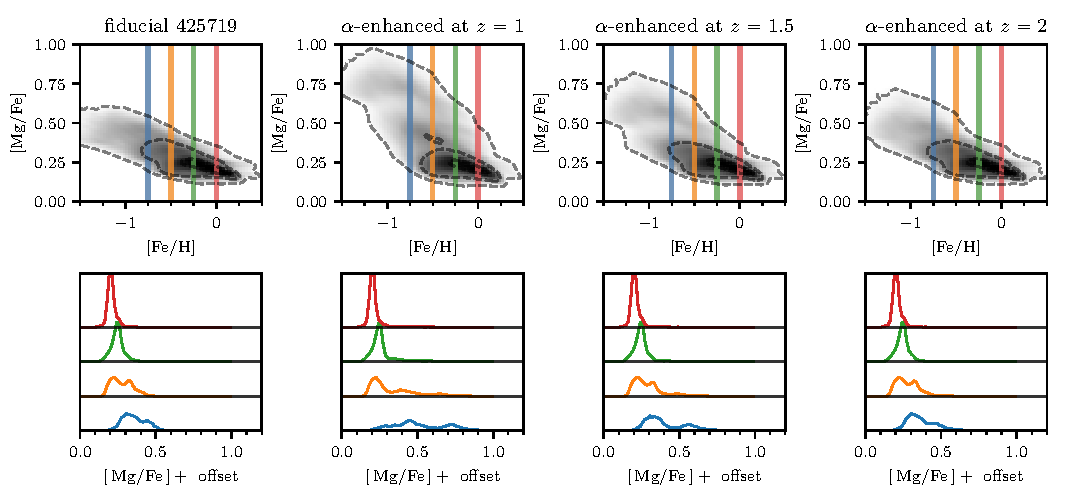
\includegraphics[width=\textwidth]{ch4/app_425719.pdf}
  \caption{The same as Figure~\ref{fig:app0}, but for a random galaxy from our initial catalog.}
  \label{fig:app10}
\end{figure*}

\begin{figure*}
  \centering
  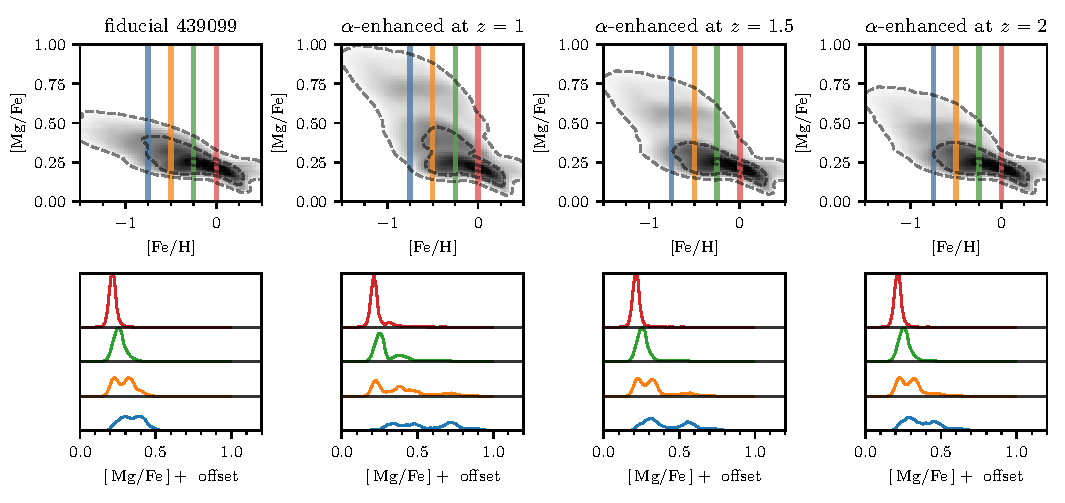
\includegraphics[width=\textwidth]{ch4/app_439099.pdf}
  \caption{The same as Figure~\ref{fig:app0}, but for a random galaxy from our initial catalog.}
  \label{fig:app11}
\end{figure*}

\begin{figure*}
  \centering
  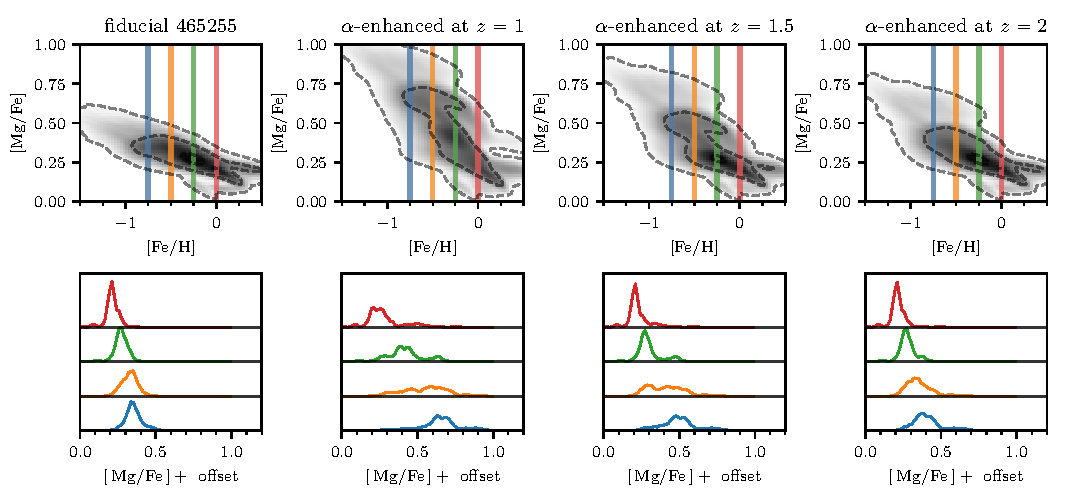
\includegraphics[width=\textwidth]{ch4/app_465255.pdf}
  \caption{The same as Figure~\ref{fig:app0}, but for a random galaxy from our initial catalog.}
  \label{fig:app12}
\end{figure*}

\begin{figure*}
  \centering
  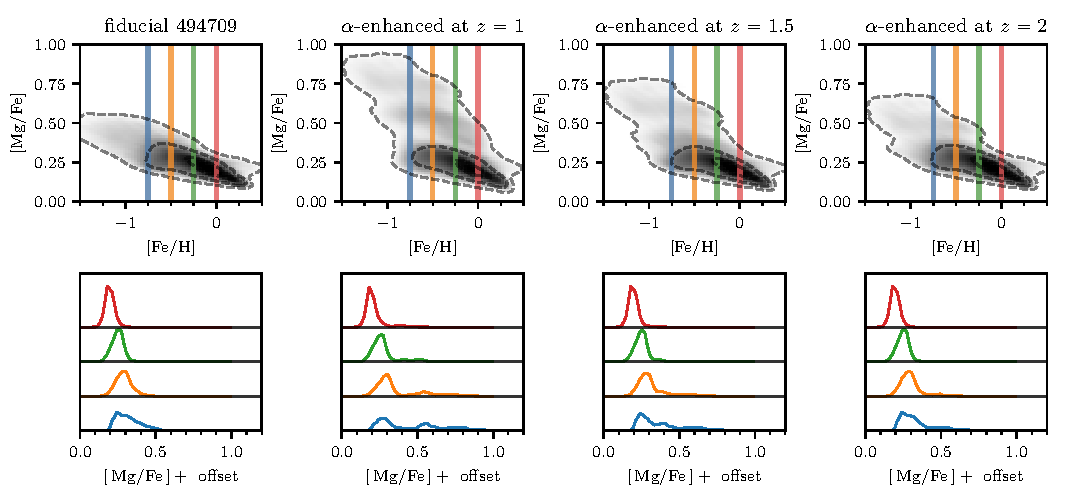
\includegraphics[width=\textwidth]{ch4/app_494709.pdf}
  \caption{The same as Figure~\ref{fig:app0}, but for a random galaxy from our initial catalog.}
  \label{fig:app13}
\end{figure*}

\begin{figure*}
  \centering
  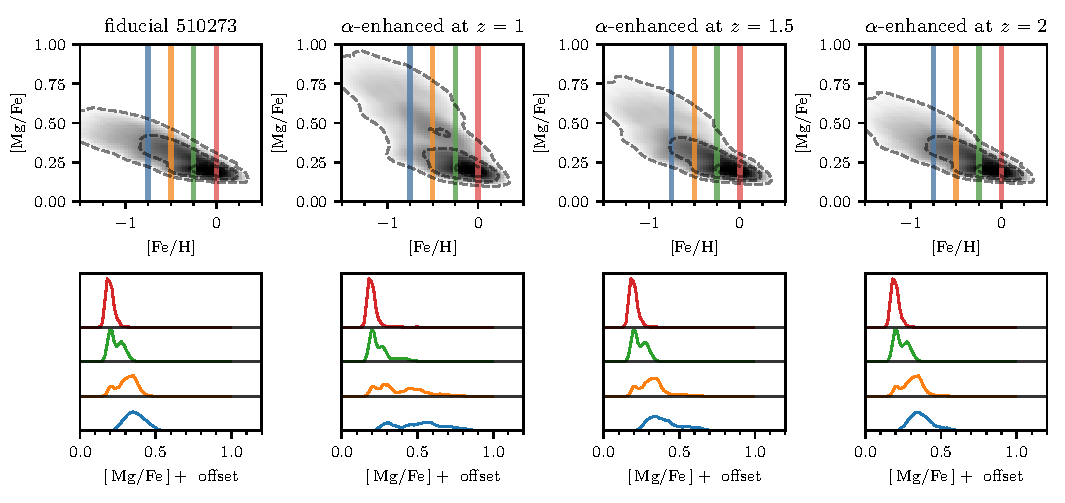
\includegraphics[width=\textwidth]{ch4/app_510273.pdf}
  \caption{The same as Figure~\ref{fig:app0}, but for a random galaxy from our initial catalog.}
  \label{fig:app14}
\end{figure*}

\begin{figure*}
  \centering
  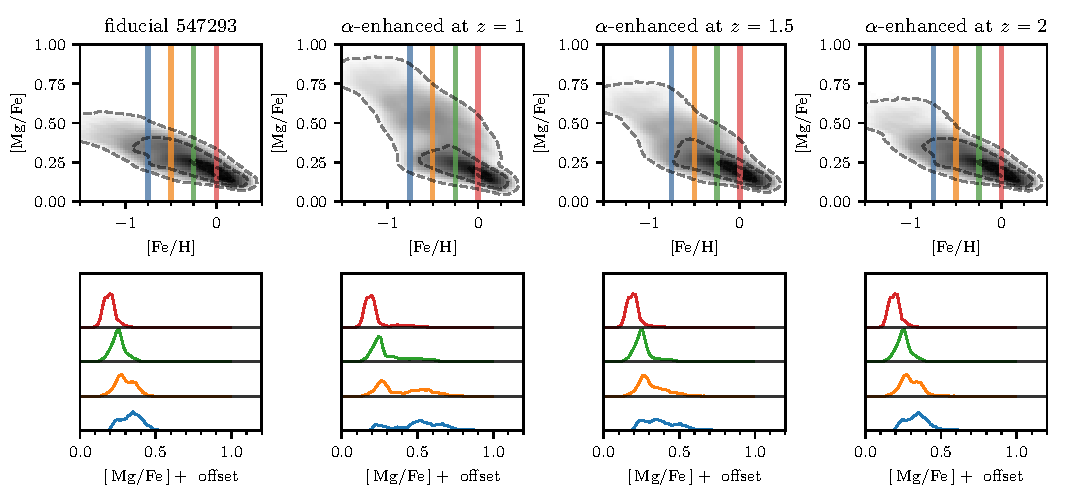
\includegraphics[width=\textwidth]{ch4/app_547293.pdf}
  \caption{The same as Figure~\ref{fig:app0}, but for a random galaxy from our initial catalog.}
  \label{fig:app15}
\end{figure*}

\begin{figure*}
  \centering
  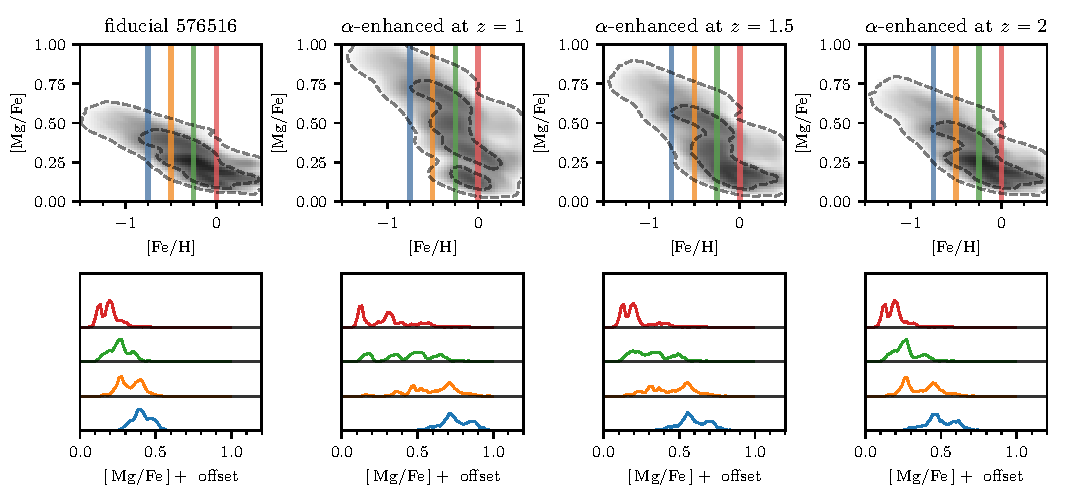
\includegraphics[width=\textwidth]{ch4/app_576516.pdf}
  \caption{The same as Figure~\ref{fig:app0}, but for a random galaxy from our initial catalog.}
  \label{fig:app16}
\end{figure*}

\chapter{The Emergence of Human Consciousness}
\begin{adjustwidth}{.8cm}{0cm}
\textit{Three things can not hide for long: the Moon, the Sun and the Truth.}

\hspace{9cm} -- Siddhartha Gautama
\end{adjustwidth}

\noindent
We now broaden our interests considerably. One of the great mysteries of our time is that the sun and moon have approximately the same apparent diameter on the sky, an apparent coincidence. However, because the moon is receding from the Earth, a more precise statement is that the coincidence is between the timing of the emergence of human consciousness at a time when the sun and moon have the same apparent diameter.

A natural outcome of the similar size of the sun and moon is the presence of total solar eclipses. However, because they have such similar sizes on the sky, total solar eclipses are quite rare, occurring about once every 375 years for a given spot on Earth \citep[varying somewhat with latitude][]{2002mmam.book.....M}. Given the current recession rate of the moon of $\sim3.8\,\textrm{cm}/\textrm{yr}$, the semi-major axis of the moon would have been $\sim0.02\,\%$ smaller when \textit{Homo erectus} emerged $\sim2\,\Myr$ ago, implying a very minor change to the overall occurrence of total solar eclipses. Assuming a generational turnover of $20\,\textrm{yr}$ \citep{homoerectus_lifespan}, this means that \textit{H. erectus} on average witnessed a solar eclipse about once every 18 generations.\footnote{This estimate is agnostic to whether they had a nomadic or sedentary lifestyle, since any movement patterns would be uncorrelated with impending eclipses. Note also that a given lineage from $2\,\Myr$ ago to the present would encounter about 5k eclipses, assuming 20~years between each generation.} This begs the question of how they would interpret such an event, and if it may lead to any appreciable effect on their long-term evolutionary outcome.

The answer is likely not, but it is even more likely that no one is still reading, so we can continue. Does witnessing totality confer any advantage for the emergence of consciousness? Because there is no genetic bias towards who would witness an eclipse, the effect must be of second-order. As an illustrative example, the attempt of a small child to understand an eclipse might push their brain to develop a slightly higher mental capacity. Some children will be able to develop this capacity at a higher rate than others because of random genetic mutations, and it is those children who are conferred an evolutionary advantage. The fact these events happen on generational timescales only enforce their power.

To be clear, this proposition is by no means a direct cause and effect argument. It is clearly not the case that consciousness emerged during the first-ever solar eclipse. However, the fact that the sun and moon have the same apparent size on the sky, and that solar eclipses happen regularly but with an occurrence that makes them a powerful and mysterious event, may have made the arising of consciousness go from being a $20\sigma$ event to an $18\sigma$ event.

\end{appendices}


\end{document}
